%%%%%%%%%%%%%%%%%%%%%%%%%%%%%%%%%%%%%%%%%
% The Legrand Orange Book
% LaTeX Template
% Version 2.0 (9/2/15)
%
% This template has been downloaded from:
% http://www.LaTeXTemplates.com
%
% Mathias Legrand (legrand.mathias@gmail.com) with modifications by:
% Vel (vel@latextemplates.com)
%
% License:
% CC BY-NC-SA 3.0 (http://creativecommons.org/licenses/by-nc-sa/3.0/)
%
% Compiling this template:
% This template uses biber for its bibliography and makeindex for its index.
% When you first open the template, compile it from the command line with the 
% commands below to make sure your LaTeX distribution is configured correctly:
%
% 1) pdflatex main
% 2) makeindex main.idx -s StyleInd.ist
% 3) biber main
% 4) pdflatex main x 2
%
% After this, when you wish to update the bibliography/index use the appropriate
% command above and make sure to compile with pdflatex several times 
% afterwards to propagate your changes to the document.
%
% This template also uses a number of packages which may need to be
% updated to the newest versions for the template to compile. It is strongly
% recommended you update your LaTeX distribution if you have any
% compilation errors.
%
% Important note:
% Chapter heading images should have a 2:1 width:height ratio,
% e.g. 920px width and 460px height.
%
%%%%%%%%%%%%%%%%%%%%%%%%%%%%%%%%%%%%%%%%%

%----------------------------------------------------------------------------------------
%	PACKAGES AND OTHER DOCUMENT CONFIGURATIONS
%----------------------------------------------------------------------------------------

\documentclass[11pt,fleqn]{book} % Default font size and left-justified equations
\usepackage{float}% para ter [H]


\usepackage[dvipsnames*,svgnames]{xcolor}
\definecolor{lowgray}{RGB}{240,240,240}

\usepackage[most]{tcolorbox}
\newtcolorbox{lattention}{breakable,enhanced,arc=0mm,colback=gray!5,colframe=gray,leftrule=12mm,%
overlay={\node[anchor=north west,outer sep=2pt] at (frame.north west) {
\includegraphics[width=8mm]{Pictures/attention2.png}}; }}


\usepackage{fancyvrb}


\usepackage[generate,ps2eps]{abc}%%sudo apt-get install abcm2ps

\usepackage[nointegrals]{wasysym}
\usepackage{harmony}
%----------------------------------------------------------------------------------------

%%%%%%%%%%%%%%%%%%%%%%%%%%%%%%%%%%%%%%%%%
% The Legrand Orange Book
% Structural Definitions File
% Version 2.0 (9/2/15)
%
% Original author:
% Mathias Legrand (legrand.mathias@gmail.com) with modifications by:
% Vel (vel@latextemplates.com)
% 
% This file has been downloaded from:
% http://www.LaTeXTemplates.com
%
% License:
% CC BY-NC-SA 3.0 (http://creativecommons.org/licenses/by-nc-sa/3.0/)
%
%%%%%%%%%%%%%%%%%%%%%%%%%%%%%%%%%%%%%%%%%

%----------------------------------------------------------------------------------------
%	VARIOUS REQUIRED PACKAGES AND CONFIGURATIONS
%----------------------------------------------------------------------------------------


\usepackage{tikz} % Required for drawing custom shapes


\usepackage{enumitem} % Customize lists
\setlist{nolistsep} % Reduce spacing between bullet points and numbered lists

\usepackage{booktabs} % Required for nicer horizontal rules in tables




%----------------------------------------------------------------------------------------
%	FONTS
%----------------------------------------------------------------------------------------

\usepackage{avant} % Use the Avantgarde font for headings
%\usepackage{times} % Use the Times font for headings
\usepackage{mathptmx} % Use the Adobe Times Roman as the default text font together with math symbols from the Sym­bol, Chancery and Com­puter Modern fonts

\usepackage{microtype} % Slightly tweak font spacing for aesthetics
\usepackage[utf8]{inputenc} % Required for including letters with accents
\usepackage[T1]{fontenc} % Use 8-bit encoding that has 256 glyphs



%----------------------------------------------------------------------------------------
%	MAIN TABLE OF CONTENTS
%----------------------------------------------------------------------------------------

\usepackage{titletoc} % Required for manipulating the table of contents

\contentsmargin{0cm} % Removes the default margin

% Part text styling
\titlecontents{part}[0cm]
{\addvspace{20pt}\centering\large\bfseries}
{}
{}
{}

% Chapter text styling
\titlecontents{chapter}[1.25cm] % Indentation
{\addvspace{12pt}\large\sffamily\bfseries} % Spacing and font options for chapters
{\color{ocre!60}\contentslabel[\Large\thecontentslabel]{1.25cm}\color{ocre}} % Chapter number
{\color{ocre}}  
{\color{ocre!60}\normalsize\;\titlerule*[.5pc]{.}\;\thecontentspage} % Page number

% Section text styling
\titlecontents{section}[2.00cm] % Indentation
{\addvspace{3pt}\sffamily\bfseries} % Spacing and font options for sections
{\contentslabel[\thecontentslabel]{1.25cm}} % Section number
{}
{\hfill\color{black}\thecontentspage} % Page number
[]

% Subsection text styling
\titlecontents{subsection}[2.00cm] % Indentation
{\addvspace{1pt}\sffamily\small} % Spacing and font options for subsections
{\contentslabel[\thecontentslabel]{1.25cm}} % Subsection number
{}
{\ \titlerule*[.5pc]{.}\;\thecontentspage} % Page number
[]

% List of figures
\titlecontents{figure}[0em]
{\addvspace{-5pt}\sffamily}
{\thecontentslabel\hspace*{1em}}
{}
{\ \titlerule*[.5pc]{.}\;\thecontentspage}
[]

% List of tables
\titlecontents{table}[0em]
{\addvspace{-5pt}\sffamily}
{\thecontentslabel\hspace*{1em}}
{}
{\ \titlerule*[.5pc]{.}\;\thecontentspage}
[]

%----------------------------------------------------------------------------------------
%	MINI TABLE OF CONTENTS IN PART HEADS
%----------------------------------------------------------------------------------------

% Chapter text styling
\titlecontents{lchapter}[0em] % Indenting
{\addvspace{15pt}\large\sffamily\bfseries} % Spacing and font options for chapters
{\color{ocre}\contentslabel[\Large\thecontentslabel]{1.25cm}\color{ocre}} % Chapter number
{}  
{\color{ocre}\normalsize\sffamily\bfseries\;\titlerule*[.5pc]{.}\;\thecontentspage} % Page number

% Section text styling
\titlecontents{lsection}[0em] % Indenting
{\sffamily\small} % Spacing and font options for sections
{\contentslabel[\thecontentslabel]{1.25cm}} % Section number
{}
{}

% Subsection text styling
\titlecontents{lsubsection}[.5em] % Indentation
{\normalfont\footnotesize\sffamily} % Font settings
{}
{}
{}

%----------------------------------------------------------------------------------------
%	PAGE HEADERS
%----------------------------------------------------------------------------------------

\usepackage{fancyhdr} % Required for header and footer configuration

\pagestyle{fancy}
\renewcommand{\chaptermark}[1]{\markboth{\sffamily\normalsize\bfseries\chaptername\ \thechapter.\ #1}{}} % Chapter text font settings
\renewcommand{\sectionmark}[1]{\markright{\sffamily\normalsize\thesection\hspace{5pt}#1}{}} % Section text font settings
\fancyhf{} \fancyhead[LE,RO]{\sffamily\normalsize\thepage} % Font setting for the page number in the header
\fancyhead[LO]{\rightmark} % Print the nearest section name on the left side of odd pages
\fancyhead[RE]{\leftmark} % Print the current chapter name on the right side of even pages
\renewcommand{\headrulewidth}{0.5pt} % Width of the rule under the header
\addtolength{\headheight}{2.5pt} % Increase the spacing around the header slightly
\renewcommand{\footrulewidth}{0pt} % Removes the rule in the footer
\fancypagestyle{plain}{\fancyhead{}\renewcommand{\headrulewidth}{0pt}} % Style for when a plain pagestyle is specified

% Removes the header from odd empty pages at the end of chapters
\makeatletter
\renewcommand{\cleardoublepage}{
\clearpage\ifodd\c@page\else
\hbox{}
\vspace*{\fill}
\thispagestyle{empty}
\newpage
\fi}

%----------------------------------------------------------------------------------------
%	DEFINITION OF THEOREM BOXES
%----------------------------------------------------------------------------------------
\usepackage{amsmath,amsfonts,amssymb,amsthm} % For math equations, theorems, symbols, etc

\newcommand{\intoo}[2]{\mathopen{]}#1\,;#2\mathclose{[}}
\newcommand{\ud}{\mathop{\mathrm{{}d}}\mathopen{}}
\newcommand{\intff}[2]{\mathopen{[}#1\,;#2\mathclose{]}}
\newtheorem{notation}{Notation}[chapter]

% Boxed/framed environments
\newtheoremstyle{ocrenumbox}% % Theorem style name
{0pt}% Space above
{0pt}% Space below
{\normalfont}% % Body font
{}% Indent amount
{\small\bf\sffamily\color{ocre}}% % Theorem head font
{\;}% Punctuation after theorem head
{0.25em}% Space after theorem head
{\small\sffamily\color{ocre}\thmname{#1}\nobreakspace\thmnumber{\@ifnotempty{#1}{}\@upn{#2}}% Theorem text (e.g. Theorem 2.1)
\thmnote{\nobreakspace\the\thm@notefont\sffamily\bfseries\color{black}---\nobreakspace#3}} % Optional theorem note
\renewcommand{\qedsymbol}{$\blacksquare$}% Optional qed square

\newtheoremstyle{blacknumex}% Theorem style name
{5pt}% Space above
{5pt}% Space below
{\normalfont}% Body font
{} % Indent amount
{\small\bf\sffamily}% Theorem head font
{\;}% Punctuation after theorem head
{0.25em}% Space after theorem head
{\small\sffamily{\tiny\ensuremath{\blacksquare}}\nobreakspace\thmname{#1}\nobreakspace\thmnumber{\@ifnotempty{#1}{}\@upn{#2}}% Theorem text (e.g. Theorem 2.1)
\thmnote{\nobreakspace\the\thm@notefont\sffamily\bfseries---\nobreakspace#3}}% Optional theorem note

\newtheoremstyle{blacknumbox} % Theorem style name
{0pt}% Space above
{0pt}% Space below
{\normalfont}% Body font
{}% Indent amount
{\small\bf\sffamily}% Theorem head font
{\;}% Punctuation after theorem head
{0.25em}% Space after theorem head
{\small\sffamily\thmname{#1}\nobreakspace\thmnumber{\@ifnotempty{#1}{}\@upn{#2}}% Theorem text (e.g. Theorem 2.1)
\thmnote{\nobreakspace\the\thm@notefont\sffamily\bfseries---\nobreakspace#3}}% Optional theorem note

% Non-boxed/non-framed environments
\newtheoremstyle{ocrenum}% % Theorem style name
{5pt}% Space above
{5pt}% Space below
{\normalfont}% % Body font
{}% Indent amount
{\small\bf\sffamily\color{ocre}}% % Theorem head font
{\;}% Punctuation after theorem head
{0.25em}% Space after theorem head
{\small\sffamily\color{ocre}\thmname{#1}\nobreakspace\thmnumber{\@ifnotempty{#1}{}\@upn{#2}}% Theorem text (e.g. Theorem 2.1)
\thmnote{\nobreakspace\the\thm@notefont\sffamily\bfseries\color{black}---\nobreakspace#3}} % Optional theorem note
\renewcommand{\qedsymbol}{$\blacksquare$}% Optional qed square
\makeatother

% Defines the theorem text style for each type of theorem to one of the three styles above
\newcounter{dummy} 
\numberwithin{dummy}{section}
\theoremstyle{ocrenumbox}
\newtheorem{theoremeT}[dummy]{Theorem}
\newtheorem{problem}{Problem}[chapter]
\newtheorem{exerciseT}{Exercise}[chapter]
\theoremstyle{blacknumex}
\newtheorem{exampleT}{Exemplo}[chapter]
\theoremstyle{blacknumbox}
\newtheorem{vocabulary}{Vocabulary}[chapter]
\newtheorem{definitionT}{Definição}[chapter]
\newtheorem{corollaryT}[dummy]{Corollary}
\theoremstyle{ocrenum}
\newtheorem{proposition}[dummy]{Proposition}

%----------------------------------------------------------------------------------------
%	DEFINITION OF COLORED THEOREM BOXES
%----------------------------------------------------------------------------------------

\RequirePackage[framemethod=default]{mdframed} % Required for creating the theorem, definition, exercise and corollary boxes

% Theorem box
\newmdenv[skipabove=7pt,
skipbelow=7pt,
backgroundcolor=black!5,
linecolor=ocre,
innerleftmargin=5pt,
innerrightmargin=5pt,
innertopmargin=5pt,
leftmargin=0cm,
rightmargin=0cm,
innerbottommargin=5pt]{tBox}

% Exercise box	  
\newmdenv[skipabove=7pt,
skipbelow=7pt,
rightline=false,
leftline=true,
topline=false,
bottomline=false,
backgroundcolor=ocre!10,
linecolor=ocre,
innerleftmargin=5pt,
innerrightmargin=5pt,
innertopmargin=5pt,
innerbottommargin=5pt,
leftmargin=0cm,
rightmargin=0cm,
linewidth=4pt]{eBox}	

% Definition box
\newmdenv[skipabove=7pt,
skipbelow=7pt,
rightline=false,
leftline=true,
topline=false,
bottomline=false,
linecolor=ocre,
innerleftmargin=5pt,
innerrightmargin=5pt,
innertopmargin=0pt,
leftmargin=0cm,
rightmargin=0cm,
linewidth=4pt,
innerbottommargin=0pt]{dBox}	

% Corollary box
\newmdenv[skipabove=7pt,
skipbelow=7pt,
rightline=false,
leftline=true,
topline=false,
bottomline=false,
linecolor=gray,
backgroundcolor=black!5,
innerleftmargin=5pt,
innerrightmargin=5pt,
innertopmargin=5pt,
leftmargin=0cm,
rightmargin=0cm,
linewidth=4pt,
innerbottommargin=5pt]{cBox}

% Creates an environment for each type of theorem and assigns it a theorem text style from the "Theorem Styles" section above and a colored box from above
\newenvironment{theorem}{\begin{tBox}\begin{theoremeT}}{\end{theoremeT}\end{tBox}}
\newenvironment{exercise}{\begin{eBox}\begin{exerciseT}}{\hfill{\color{ocre}\tiny\ensuremath{\blacksquare}}\end{exerciseT}\end{eBox}}				  
\newenvironment{definition}{\begin{dBox}\begin{definitionT}}{\end{definitionT}\end{dBox}}	
\newenvironment{example}{\begin{exampleT}}{\hfill{\tiny\ensuremath{\blacksquare}}\end{exampleT}}		
\newenvironment{corollary}{\begin{cBox}\begin{corollaryT}}{\end{corollaryT}\end{cBox}}	

%----------------------------------------------------------------------------------------
%	REMARK ENVIRONMENT
%----------------------------------------------------------------------------------------
\newenvironment{remark}{\par\vspace{10pt}\small % Vertical white space above the remark and smaller font size
\begin{list}{}{
\leftmargin=35pt % Indentation on the left
\rightmargin=25pt}\item\ignorespaces % Indentation on the right
\makebox[-2.5pt]{\begin{tikzpicture}[overlay]
\node[draw=ocre!60,line width=1pt,circle,fill=ocre!25,font=\sffamily\bfseries,inner sep=2pt,outer sep=0pt] at (-15pt,0pt){\textcolor{ocre}{R}};\end{tikzpicture}} % Orange R in a circle
\advance\baselineskip -1pt}{\end{list}\vskip5pt} % Tighter line spacing and white space after remark

%----------------------------------------------------------------------------------------
%	SECTION NUMBERING IN THE MARGIN
%----------------------------------------------------------------------------------------
\makeatletter
\renewcommand{\@seccntformat}[1]{\llap{\textcolor{ocre}{\csname the#1\endcsname}\hspace{1em}}}                    
\renewcommand{\section}{\@startsection{section}{1}{\z@}
{-4ex \@plus -1ex \@minus -.4ex}
{1ex \@plus.2ex }
{\normalfont\large\sffamily\bfseries}}
\renewcommand{\subsection}{\@startsection {subsection}{2}{\z@}
{-3ex \@plus -0.1ex \@minus -.4ex}
{0.5ex \@plus.2ex }
{\normalfont\sffamily\bfseries}}
\renewcommand{\subsubsection}{\@startsection {subsubsection}{3}{\z@}
{-2ex \@plus -0.1ex \@minus -.2ex}
{.2ex \@plus.2ex }
{\normalfont\small\sffamily\bfseries}}                        
\renewcommand\paragraph{\@startsection{paragraph}{4}{\z@}
{-2ex \@plus-.2ex \@minus .2ex}
{.1ex}
{\normalfont\small\sffamily\bfseries}}

%----------------------------------------------------------------------------------------
%	PART HEADINGS
%----------------------------------------------------------------------------------------

% numbered part in the table of contents
\newcommand{\@mypartnumtocformat}[2]{%
\setlength\fboxsep{0pt}%
\noindent\colorbox{ocre!20}{\strut\parbox[c][.7cm]{\ecart}{\color{ocre!70}\Large\sffamily\bfseries\centering#1}}\hskip\esp\colorbox{ocre!40}{\strut\parbox[c][.7cm]{\linewidth-\ecart-\esp}{\Large\sffamily\centering#2}}}%
%%%%%%%%%%%%%%%%%%%%%%%%%%%%%%%%%%
% unnumbered part in the table of contents
\newcommand{\@myparttocformat}[1]{%
\setlength\fboxsep{0pt}%
\noindent\colorbox{ocre!40}{\strut\parbox[c][.7cm]{\linewidth}{\Large\sffamily\centering#1}}}%
%%%%%%%%%%%%%%%%%%%%%%%%%%%%%%%%%%
\newlength\esp
\setlength\esp{4pt}
\newlength\ecart
\setlength\ecart{1.2cm-\esp}
\newcommand{\thepartimage}{}%
\newcommand{\partimage}[1]{\renewcommand{\thepartimage}{#1}}%
\def\@part[#1]#2{%
\ifnum \c@secnumdepth >-2\relax%
\refstepcounter{part}%
\addcontentsline{toc}{part}{\texorpdfstring{\protect\@mypartnumtocformat{\thepart}{#1}}{\partname~\thepart\ ---\ #1}}
\else%
\addcontentsline{toc}{part}{\texorpdfstring{\protect\@myparttocformat{#1}}{#1}}%
\fi%
\startcontents%
\markboth{}{}%
{\thispagestyle{empty}%
\begin{tikzpicture}[remember picture,overlay]%
\node at (current page.north west){\begin{tikzpicture}[remember picture,overlay]%	
\fill[ocre!20](0cm,0cm) rectangle (\paperwidth,-\paperheight);
\node[anchor=north] at (4cm,-3.25cm){\color{ocre!40}\fontsize{220}{100}\sffamily\bfseries\@Roman\c@part}; 
\node[anchor=south east] at (\paperwidth-1cm,-\paperheight+1cm){\parbox[t][][t]{8.5cm}{
\printcontents{l}{0}{\setcounter{tocdepth}{1}}%
}};
\node[anchor=north east] at (\paperwidth-1.5cm,-3.25cm){\parbox[t][][t]{15cm}{\strut\raggedleft\color{white}\fontsize{30}{30}\sffamily\bfseries#2}};
\end{tikzpicture}};
\end{tikzpicture}}%
\@endpart}
\def\@spart#1{%
\startcontents%
\phantomsection
{\thispagestyle{empty}%
\begin{tikzpicture}[remember picture,overlay]%
\node at (current page.north west){\begin{tikzpicture}[remember picture,overlay]%	
\fill[ocre!20](0cm,0cm) rectangle (\paperwidth,-\paperheight);
\node[anchor=north east] at (\paperwidth-1.5cm,-3.25cm){\parbox[t][][t]{15cm}{\strut\raggedleft\color{white}\fontsize{30}{30}\sffamily\bfseries#1}};
\end{tikzpicture}};
\end{tikzpicture}}
\addcontentsline{toc}{part}{\texorpdfstring{%
\setlength\fboxsep{0pt}%
\noindent\protect\colorbox{ocre!40}{\strut\protect\parbox[c][.7cm]{\linewidth}{\Large\sffamily\protect\centering #1\quad\mbox{}}}}{#1}}%
\@endpart}
\def\@endpart{\vfil\newpage
\if@twoside
\if@openright
\null
\thispagestyle{empty}%
\newpage
\fi
\fi
\if@tempswa
\twocolumn
\fi}

%----------------------------------------------------------------------------------------
%	CHAPTER HEADINGS
%----------------------------------------------------------------------------------------
\newcommand{\thechapterimage}{}%
\newcommand{\chapterimage}[1]{\renewcommand{\thechapterimage}{#1}}%
\def\@makechapterhead#1{%
{\parindent \z@ \raggedright \normalfont
\ifnum \c@secnumdepth >\m@ne
\if@mainmatter
\begin{tikzpicture}[remember picture,overlay]
\node at (current page.north west)
{\begin{tikzpicture}[remember picture,overlay]
\node[anchor=north west,inner sep=0pt] at (0,0) {\includegraphics[width=\paperwidth]{\thechapterimage}};
\draw[anchor=west] (\Gm@lmargin,-9cm) node [line width=2pt,rounded corners=15pt,draw=ocre,fill=white,fill opacity=0.5,inner sep=15pt]{\strut\makebox[22cm]{}};
\draw[anchor=west] (\Gm@lmargin+.3cm,-9cm) node {\huge\sffamily\bfseries\color{black}\thechapter. #1\strut};
\end{tikzpicture}};
\end{tikzpicture}
\else
\begin{tikzpicture}[remember picture,overlay]
\node at (current page.north west)
{\begin{tikzpicture}[remember picture,overlay]
\node[anchor=north west,inner sep=0pt] at (0,0) {\includegraphics[width=\paperwidth]{\thechapterimage}};
\draw[anchor=west] (\Gm@lmargin,-9cm) node [line width=2pt,rounded corners=15pt,draw=ocre,fill=white,fill opacity=0.5,inner sep=15pt]{\strut\makebox[22cm]{}};
\draw[anchor=west] (\Gm@lmargin+.3cm,-9cm) node {\huge\sffamily\bfseries\color{black}#1\strut};
\end{tikzpicture}};
\end{tikzpicture}
\fi\fi\par\vspace*{270\p@}}}

%-------------------------------------------

\def\@makeschapterhead#1{%
\begin{tikzpicture}[remember picture,overlay]
\node at (current page.north west)
{\begin{tikzpicture}[remember picture,overlay]
\node[anchor=north west,inner sep=0pt] at (0,0) {\includegraphics[width=\paperwidth]{\thechapterimage}};
\draw[anchor=west] (\Gm@lmargin,-9cm) node [line width=2pt,rounded corners=15pt,draw=ocre,fill=white,fill opacity=0.5,inner sep=15pt]{\strut\makebox[22cm]{}};
\draw[anchor=west] (\Gm@lmargin+.3cm,-9cm) node {\huge\sffamily\bfseries\color{black}#1\strut};
\end{tikzpicture}};
\end{tikzpicture}
\par\vspace*{270\p@}}
\makeatother

%----------------------------------------------------------------------------------------
%	HYPERLINKS IN THE DOCUMENTS
%----------------------------------------------------------------------------------------
\usepackage{hyperref}
\hypersetup{
	hidelinks,
	backref=true,
	pagebackref=true,
	hyperindex=true,
	colorlinks=true,
	linkcolor=black,         % color of internal links (change box color with linkbordercolor)
	%pdftoolbar=true,         % show Acrobat’s toolbar?
	%pdfmenubar=true,         % show Acrobat’s menu?
	%pdffitwindow=false,      % window fit to page when opened
	%pdfstartview={FitH},     % fits the width of the page to the window
	breaklinks=true,
	urlcolor= colormylink,
	bookmarks=true,
	bookmarksopen=false,
	pdftitle={Title},
	pdfauthor={Author}
}

\usepackage{bookmark}
\bookmarksetup{
open,
numbered,
addtohook={%
\ifnum\bookmarkget{level}=0 % chapter
\bookmarksetup{bold}%
\fi
\ifnum\bookmarkget{level}=-1 % part
\bookmarksetup{color=colormylink,bold}%
\fi
}
}
 % Insert the commands.tex file which contains the majority of the structure behind the template

%%%%%%%%%%%%%%%%%%%%%%%%%%%%%%%%%%%%%%%%%%%%%%%%%%%%%%%%%%%%%%%%%%%%%%%%%%%%%%%%%%
%%%%%%%%%%%%%%%%%%%%%%%%%%%%%%%%%%%%%%%%%%%%%%%%%%%%%%%%%%%%%%%%%%%%%%%%%%%%%%%%%%
%% Modificado por Fernando Pujaico Rivera
%%%%%%%%%%%%%%%%%%%%%%%%%%%%%%%%%%%%%%%%%%%%%%%%%%%%%%%%%%%%%%%%%%%%%%%%%%%%%%%%%%
%%%%%%%%%%%%%%%%%%%%%%%%%%%%%%%%%%%%%%%%%%%%%%%%%%%%%%%%%%%%%%%%%%%%%%%%%%%%%%%%%%

%%%%%%%%%%%%%%%%%%%%%%%%%%%%%%%%%%%%
% Para \singlespacing 
\usepackage{setspace}

%%%%%%%%%%%%%%%%%%%%%%%%%%%%%%%%%%%%
% Par diferentes modelos de caption.
\usepackage{caption}
\usepackage{subcaption}

%%%%%%%%%%%%%%%%%%%%%%%%%%%%%%%%%%%%
% glossario
\usepackage{nomencl}

%%%%%%%%%%%%%%%%%%%%%%%%%%%%%%%%%%%%
% Link a referencia
\usepackage{hyperref}
\hypersetup{
   bookmarks=true,          % show bookmarks bar?
   pdftoolbar=true,         % show Acrobat’s toolbar?
   pdfmenubar=true,         % show Acrobat’s menu?
   pdffitwindow=false,      % window fit to page when opened
   pdfstartview={FitH},     % fits the width of the page to the window
   colorlinks=true,         % false: boxed links; true: colored links
   linkcolor=black,         % color of internal links (change box color with linkbordercolor)
   %citecolor=green,        % color of links to bibliography
   %filecolor=magenta,      % color of file links
   %urlcolor=cyan           % color of external links
}

%%%%%%%%%%%%%%%%%%%%%%%%%%%%%%%%%%%%
% Defino algunos colores.
\usepackage{color}
\definecolor{dkred}{rgb}{0.6,0,0}
\definecolor{dkgreen}{rgb}{0,0.6,0}
\definecolor{dkblue}{rgb}{0,0,0.6}
\definecolor{mygray}{rgb}{0.5,0.5,0.5}
\definecolor{mylowgray}{rgb}{0.9,0.9,0.9}
\definecolor{myverylowgray}{rgb}{0.95,0.95,0.95}
\definecolor{mymauve}{rgb}{0.58,0,0.82}

%%%%%%%%%%%%%%%%%%%%%%%%%%%%%%%%%%%%
% Para \lstset e insertar codigo
\usepackage{listings}
\lstset{%% configuro listings
  frame=tb,
  language=Octave,%linguagem por defeito
  captionpos=b,
  %
  aboveskip=3mm,
  belowskip=3mm,
  %backgroundcolor=\color{myverylowgray},
  showstringspaces=false,
  columns=flexible,
  basicstyle={\small\ttfamily},
  %
  numbers=none,
  numberstyle=\tiny\color{mygray},
  %
  breaklines=true,
  breakatwhitespace=true,
  tabsize=4
}

\lstdefinelanguage{OctaveMatlab}{%
  language=Octave,% Linguagem de base
  %
  classoffset=0,
  otherkeywords={..,;,=,<,>,<=,=>,==},
  keywordstyle=\color{blue},
  %  
  classoffset=1,
    morekeywords={datapack,datacut,datapack_to_gif,
		  thsp,thsp_line,thsp_random,thsp_gaussian,
		  coom,
		  pmfad,pmfrd,
		  inertiamoment,
		  avd,avd_from_data,
		  rvd,
		  fujii,gendiff,stdcont,
		  graphim,graphavd,graphrvd,graphptd,graphkurt,graphskew,
		  hbpmf,threshold2d,stscorr},
    keywordstyle=\color{dkred},
  classoffset=0,
  %
  commentstyle=\color{dkgreen},
  morecomment = [l][\itshape\color{purple!40!black}]{\%},
  %
  stringstyle=\color{mymauve},
}

\lstdefinestyle{definefunc}{%
  backgroundcolor=\color{mylowgray},
}

\lstdefinestyle{definecode}{%
  backgroundcolor=\color{myverylowgray},
}
%%%% \lstset{language=OctaveMatlab,style=definecode}%orden importa
%%%% \begin{lstlisting}
%%%%  cd directory
%%%%  ls
%%%% \end{lstlisting}

%%%%%%%%%%%%%%%%%%%%%%%%%%%%%%%%%%%%
%% Para a criação do Glossário
\makenomenclature

%%%%%%%%%%%%%%%%%%%%%%%%%%%%%%%%%%%%%%%%%%%%%%%%%%%%%%%%%%%%%%%%%%%%%%%%%%%%%%%%%%
%%%%%%%%%%%%%%%%%%%%%%%%%%%%%%%%%%%%%%%%%%%%%%%%%%%%%%%%%%%%%%%%%%%%%%%%%%%%%%%%%%
%%%%%%%%%%%%%%%%%%%%%%%%%%%%%%%%%%%%%%%%%%%%%%%%%%%%%%%%%%%%%%%%%%%%%%%%%%%%%%%%%%
%%%%%%%%%%%%%%%%%%%%%%%%%%%%%%%%%%%%%%%%%%%%%%%%%%%%%%%%%%%%%%%%%%%%%%%%%%%%%%%%%%

\begin{document}

%----------------------------------------------------------------------------------------
%	TITLE PAGE
%----------------------------------------------------------------------------------------

\begingroup
\thispagestyle{empty}
\begin{tikzpicture}[remember picture,overlay]
\coordinate [below=12cm] (midpoint) at (current page.north);
\node at (current page.north west)
{\begin{tikzpicture}[remember picture,overlay]
\node[anchor=north west,inner sep=0pt] at (0,0) {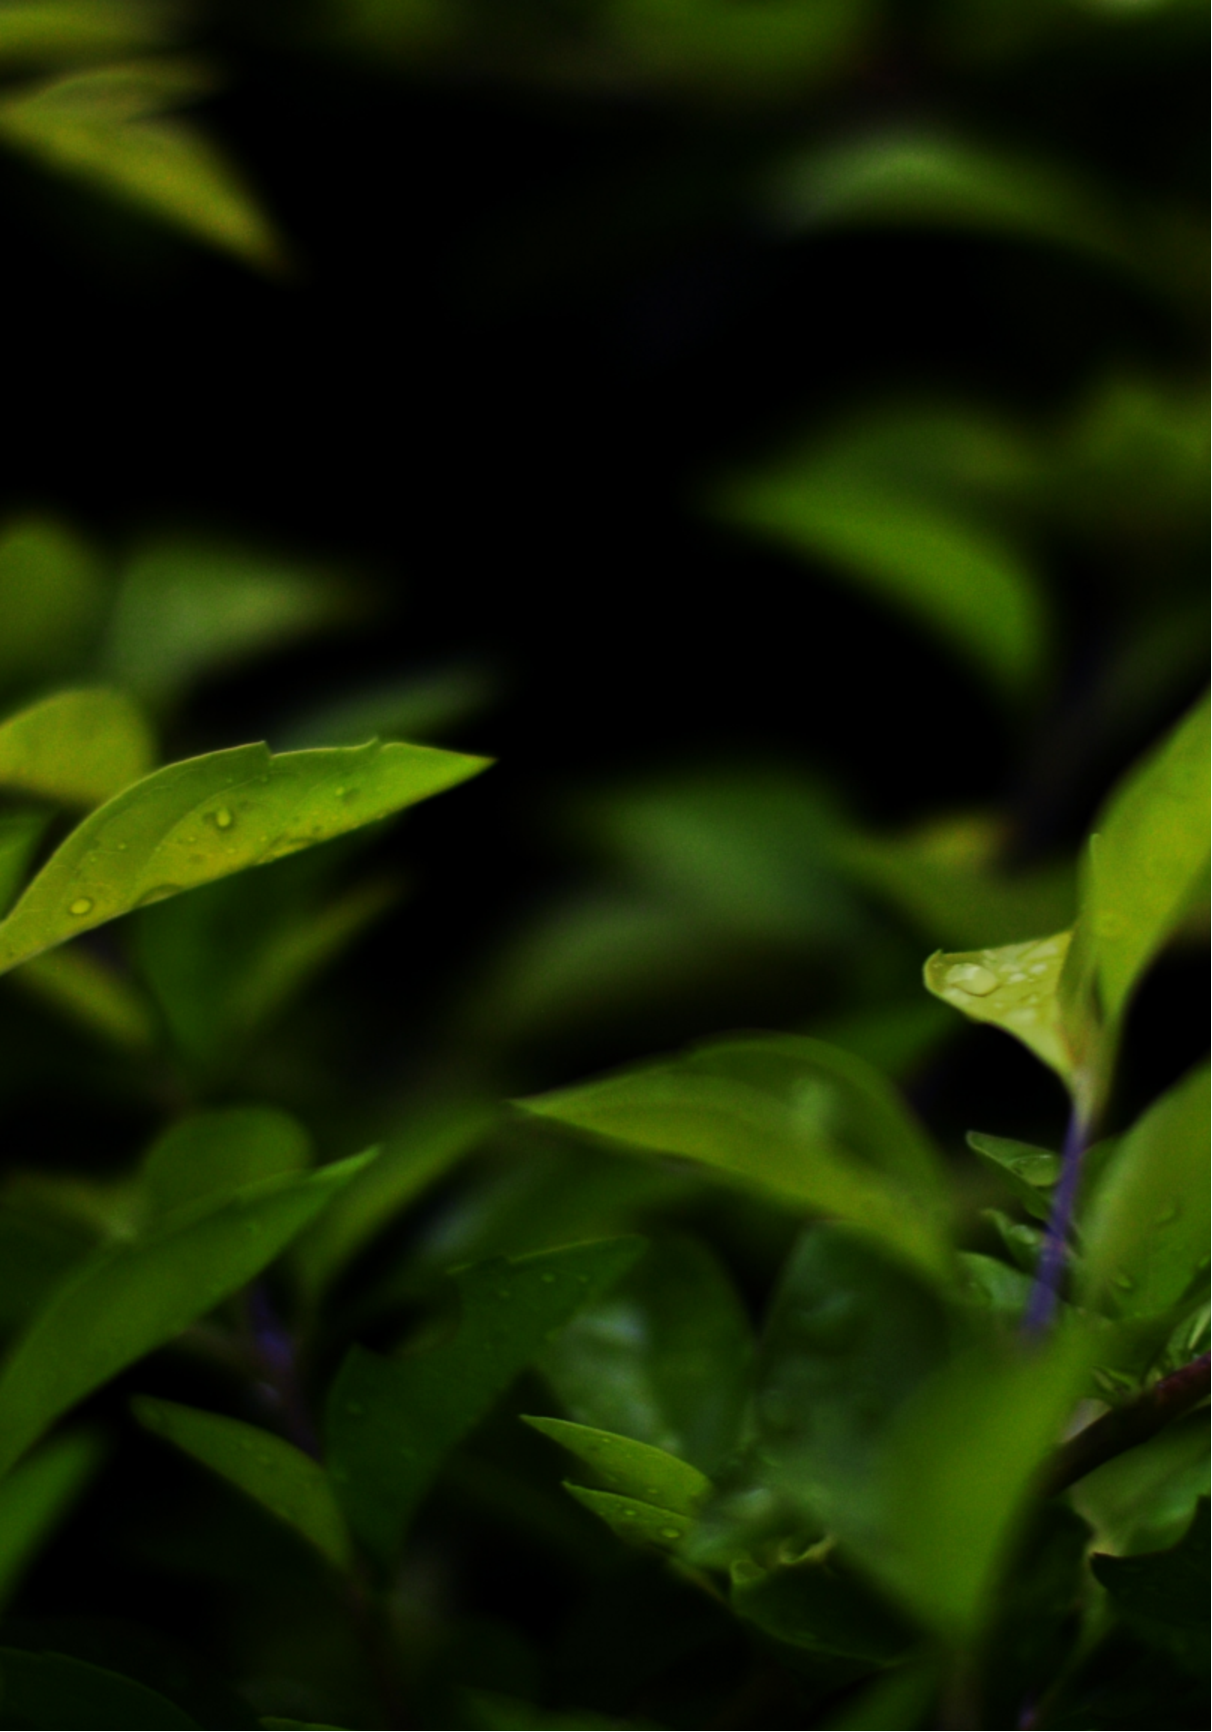
\includegraphics[width=\paperwidth]{background}}; % Background image
\draw[anchor=north] (midpoint) node [fill=ocre!30!white,fill opacity=0.6,text opacity=1,inner sep=1cm]
{\Huge\centering\bfseries\sffamily\parbox[c][][t]{\paperwidth}{\centering Partitura de movimento para samba de gafieira\\[15pt] % Book title
{\Large Uma visão particular para um público em geral}\\[20pt] % Subtitle
{\huge Fernando Pujaico Rivera}}}; % Author name
\end{tikzpicture}};
\end{tikzpicture}
\vfill
\endgroup

%----------------------------------------------------------------------------------------
%	COPYRIGHT PAGE
%----------------------------------------------------------------------------------------

\newpage
~\vfill
\thispagestyle{empty}

\noindent Copyright \copyright\ 2018 Fernando Pujaico Rivera\\ % Copyright notice

\noindent \textsc{Published by Publisher}\\ % Publisher

\noindent \textsc{book-website.com}\\ % URL

\noindent Licensed under the Creative Commons Attribution-NonCommercial 3.0 
Unported License (the ``License''). You may not use this file except in 
compliance with the License. You may obtain a copy of the License at 
\url{http://creativecommons.org/licenses/by-nc/3.0}. Unless required by 
applicable law or agreed to in writing, software distributed under the License 
is distributed on an \textsc{``as is'' basis, without warranties or conditions 
of any kind}, either express or implied. See the License for the specific 
language governing permissions and limitations under the License.\\ % License information

\noindent \textit{First printing, March 2013} % Printing/edition date

%----------------------------------------------------------------------------------------
%	TABLE OF CONTENTS
%----------------------------------------------------------------------------------------

\chapterimage{chapter_head_1.pdf} % Table of contents heading image

\pagestyle{empty} % No headers

\tableofcontents % Print the table of contents itself

\cleardoublepage % Forces the first chapter to start on an odd page so it's on the right

\pagestyle{fancy} % Print headers again

%----------------------------------------------------------------------------------------
%	PART
%----------------------------------------------------------------------------------------

\part{Introdução e fundamento teórico}

%----------------------------------------------------------------------------------------
%	CHAPTERS
%----------------------------------------------------------------------------------------
\chapterimage{chapter_head_2.pdf} % Chapter heading image

\chapter{Introdução}
%%%%%%%%%%%%%%%%%%%%%%%%%%%%%%%%%%%%%%%%%%%%%%%%%%%%%%%%%%%%%%%%%%%%%%%%%%%%%%%%
%% SECTION
%%%%%%%%%%%%%%%%%%%%%%%%%%%%%%%%%%%%%%%%%%%%%%%%%%%%%%%%%%%%%%%%%%%%%%%%%%%%%%%%
\section{Historia da samba}\index{historia da samba}
O samba é uns dos gêneros musicais mais conhecidos no Brasil do século XXI;
entre estes gêneros mais populares, temos por exemplo, ao ``forró'' e ao ``Sertanejo'';
sendo que o samba se distingue entre eles, 
como a principal expressão popular da música brasileira \cite[pp. 47]{diniz2008almanaque}. 


%O gênero samba atual é uma mistura de muitos gêneros musicais de África, América e Europa.
Porem, o caminho da palavra samba inicia muito tempo atras.
Nos inicios do seculo XIX os viajantes portugueses designavam as danças africanas com a palavra ``batuque'' \cite[pp. 54]{de4danccas},
e no Brasil existem registros desta palavra desde o século XVIII \cite[pp. 85]{sandroni2001feitico} , sendo que
esta não se usava para referenciar a uma dança em particular e sim aos festejos dos negros em geral.
Assim, a designação  ``batuque'' foi muito popular ate inícios do seculo XX, 
onde a palavra ``samba'' virou mais popular para descrever estes festejos \cite[pp. 85]{sandroni2001feitico} \cite[pp. 47]{diniz2008almanaque}; 
a Figura \ref{fig:sambacrono} descreve o uso destas palavras ao longo do tempo.
\begin{figure}[h]
  \centering
    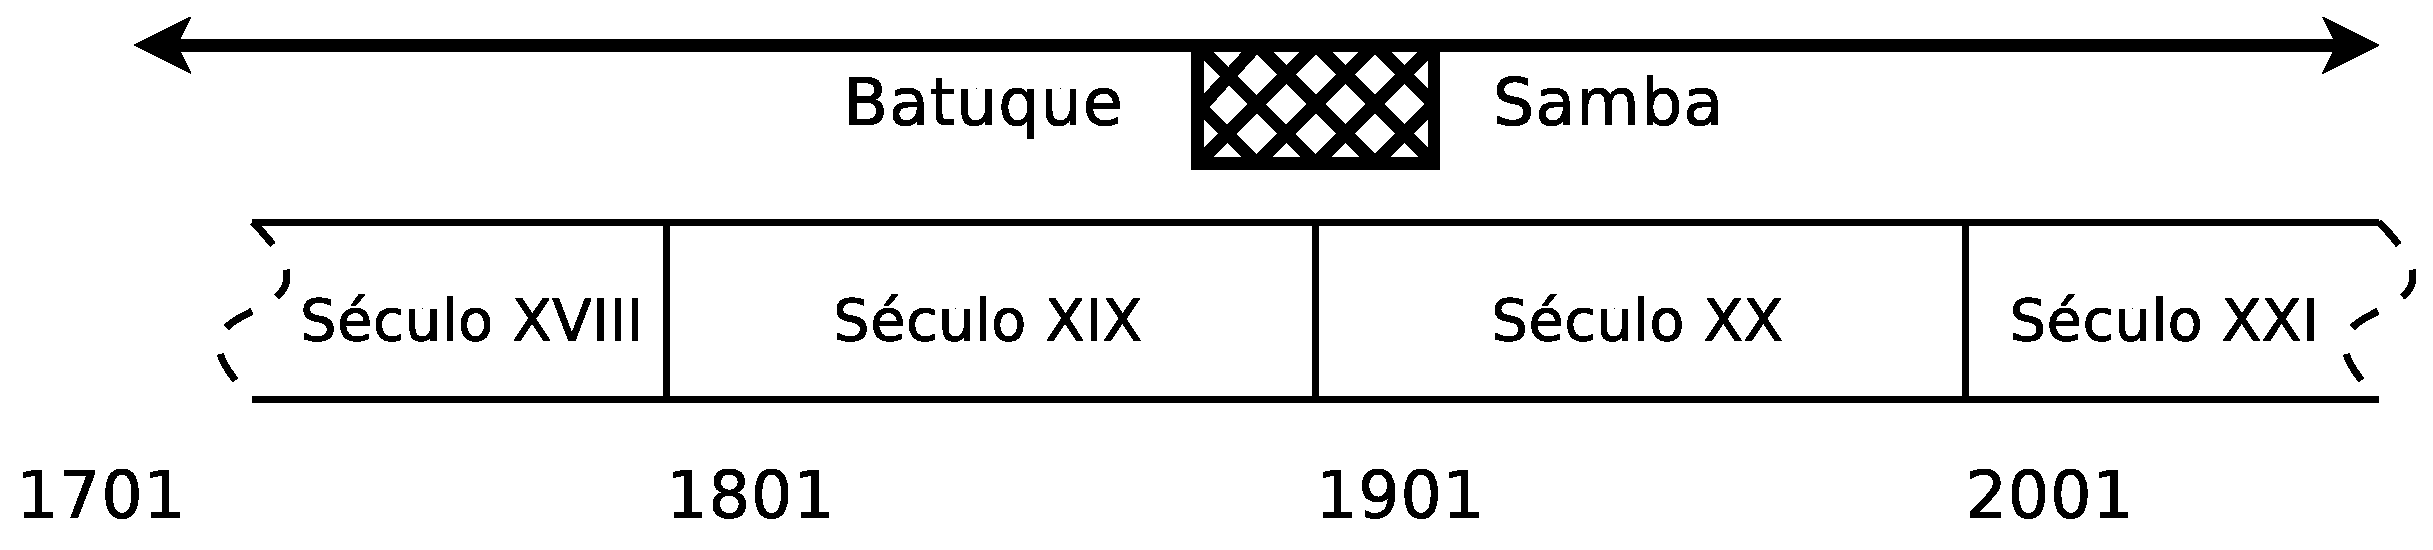
\includegraphics[width=0.85\textwidth]{chapters/cap-intro/samba-crono.eps}
  \caption{Cronologia da designação geral das danças africanas no Brasil.}
  \label{fig:sambacrono}
\end{figure}

Na literatura latino-americana a palavra ``samba'' é conhecida desde o seculo XIX, 
e no brasil desde o ano de 1838 \cite[pp. 47]{diniz2008almanaque}; porem , a palavra ``samba'' foi
quase desconhecida (em Rio de Janeiro) ate o último quartel do século XIX  \cite[pp. 86]{sandroni2001feitico}.
Entre as explicações da origem da palavra ``samba'', 
a mais conhecida, é a que promove que esta vem do idioma quimbundo, 
sendo derivado da palavra ``semba''  que significa umbigada \cite[pp. 47]{diniz2008almanaque} \cite[pp. 50]{da2015historia}.
Uma referencia muito conhecida deste vinculo é a descrita no livro ``O negro e o garimpo em Minas Gerais''
de Mata Machado Filho, onde ele comenta que ``os negros corrigem para semba se 
alguém lhes fala em samba'' \cite[pp. 85]{sandroni2001feitico}. Assim se vê que existe
desde antanho uma relação entre as palavras, 
samba, semba e umbigada.

Entre as danças "profanas" \cite[pp. 85]{sandroni2001feitico} afro-brasileiras o gesto da umbigada é um elemento muito caraterístico,
de modo que em 1961 Edson Carneiro definiu e englobou as danças que realizam este 
gesto como ``samba-de-umbigada'' . Assim tradições 
musicais como o samba de roda, o jongo, o lundu, o coco, o calango e o cateretê, 
seguindo Edson são englobadas com  ``samba-de-umbigada'' \cite[pp. 85]{sandroni2001feitico}.

%%%%%%%%%%%%%%%%%%%%%%%%%%%%%%%%%%%%%%%%%%%%%%%%%%%%%%%%%%%%%%%%%%%%%%%%%%%%%%%%
%% SECTION
%%%%%%%%%%%%%%%%%%%%%%%%%%%%%%%%%%%%%%%%%%%%%%%%%%%%%%%%%%%%%%%%%%%%%%%%%%%%%%%%
\section{Historia das gafieiras}\index{historia das gafieiras}

Desde inícios do século XX já existiam associações para negros e mestiços, 
com distintas  finalidades, entre elas estava a criação de 
"sociedades dançantes ou recreativas" abertas a um publico geral
\cite[pp. 154-155]{neres1999negro} \cite[pp. 71]{de2008bexiga} \cite[pp. 11]{respeitojournalbrasil1}.
Estas associações geralmente não tinham local próprio, 
e tinham que alugar espaços que terminavam sendo salões de velhos sobrados
ou similares \cite[pp. 154-155]{neres1999negro} \cite[pp. 49]{diniz2003almanaque}.

A que é considerada a primeira sociedade de dança, que agora definiríamos como gafieira, 
é a ``Sociedade de Danças Clovis Invencivel''\footnote{Em algumas versões 
``Clovis Invencivel'' é referenciado como ``Clowns Invencíveis'' \cite[pp. 3]{juliosimoes} ou 
``Clovis Invencíveis'' \cite[pp. 10]{simoesjournalbrasil1}}, 
foi fundada no Rio de Janeiro em 1906, 
onde eram populares concursos de valsa, polka ou quadrilha \cite[pp. 3]{entrevistajuliojournalbrasil1}.
O dono da ideia da criação destes concursos foi um muito jovem e fiscal do salão, Júlio Simões,
que a seus 16 anos pensou numa sociedade de dança diferente dos da época,
que se dedicavam a ``bater bumbo'' (bailes carnavalescos ou de zé-pereira\footnote{ Uma sociedade recreativa do ``Ze-pereira''
é uma sociedade dedicada a dança carnavalesca \cite[pp. 10]{simoesjournalbrasil1}}), 
a uma dedicada a ``arrasta-pés'' (bailes de salão) \cite[pp. 3]{entrevistajuliojournalbrasil1} \cite[pp. 3]{juliosimoes} \cite[pp. 10]{simoesjournalbrasil1}.

Com o surgir dos lugares de baile, 
Júlio Simões, e sócios, decidiram em 1914 fundar a ``Kanaga do Japão'',
lugar de grande tradição no Rio de Janeiro,
onde o conjunto encarregado de animar o local era cheifado por Sinhô e Bulhões de Carvalho,
que receberam o título popular de ``reis da valsa'',
com torneios de dança que duravam ate 55 
minutos \footnote{Informação extraída de uma entrevista a Júlio Simões realizada o 3 de Agosto de 1961, no Jornal do Brasil.} 
dançando uma valsa rápida \cite[pp. 3]{entrevistajuliojournalbrasil1}.

Para o ano 1930, estas sociedades dançantes tinham ganhado muita popularidade, e salões de dança como a
"Kananga do Japão" eram dos mais concorridos. Porem,
apos a morte de um socio da "Kananga do Japão", 
Júlio Simões se associa com Heitor Persegani, e convida para ajudá-los a Hilário Jovino, 
e decidem fundar o local de danças chamado "Elite club" \cite[pp. 11]{eliteinaugura},
agora chamado "Elite clube" \cite[pp. 3]{juliosimoes},
na Rua Frei Caneca n. 4 - Centro, Rio de Janeiro - RJ;
sendo o 17 de julho de 1930 seu baile inaugural 
\cite[pp. 11]{eliteinaugura} \cite[pp. 3]{juliosimoes} \cite[pp. 10]{simoesjournalbrasil1}.

Uma descrição de uma destas sociedades dançantes, pode ser vista no livro "O cabrocha"; 
escrita  por Jota Efegê em 1931; 
sobre a "Sociedade Recreativa Familiar Bohemios de Botafogo" [pp. 24-26]\cite{jotaefege},
a continuação é mostrado um extracto desse texto:
\begin{tcolorbox}[breakable,colback=lowgray,colframe=lowgray]%%
O salão, comquanto não fosse de grandes dimensões, era
de um tamanho regular, confinando com uma pequena saleta
onde tambem se dansava; estava bem affluido. Numa
heterogeneidade foliã, via-se desde a crioulinha blasée, sem
elegancia, desalinhada, á mulatinha pernostica de faces
avermelhadas por um carmin berrante, cabello engommado e
subjugado por travessas e grampos, num á la garçonne
forçado, mas exigido pela moda. Em meio dessas "cabrochas"
e "roxinhas", viam-se algumas moças brancas de apparencia
sobria. São as meninas que não podem fazer um vestido de
seda ou calçar sapatos de setim, para se apresentarem no
Fluminense ou no Flamengo e que nestes clubes se divertem,
ficando em evidencia por serem brancas.  %~\\
(Jota Efegê)
\end{tcolorbox}



O termo gafieira foi criado pelo cronista carnavalesco, 
Romeu Arêde\footnote{Em algumas versões está mal referenciado como Romeu Aredo \cite[pp. 188]{raca1999}.}, 
também conhecido como "Picareta" \cite[pp. 3]{juliosimoes} \cite[pp. 21]{efege1974maxixe} \cite[pp. 78]{coutinho2006cronistas}, 
colunista da seção recreativa do ``Jornal do Brasil'' \cite[pp. 18]{entrevistajuliojournalbrasil1}.
Júlio Simões afirma que o jornalista tinha a costume de entrar, comer, beber, dançar e não pagar,
e que quando ele impediu o ingresso ao jornalista e seus acompanhantes à voz: ``Aqui tem ordem'' \cite[pp.13 ]{respeitojournalbrasil1},
indicando que só podiam entrar com entrada franca ele mais uma dama ou um amigo,
o cronista reagiu indicando a seus acompanhantes a se retirarem, exclamando: 
``Vamos embora! Isto aqui é uma gafieira!'' \cite[pp. 29]{instituto1987revista};
Ao dia seguinte no Jornal do Brasil, Picareta escreveria:
``Aquele é um lugar da ralé, onde se cometem gafes em fieiras''\footnote{Na 
revista Raça Brasil se indica que este incidente aconteceu em 1932 \cite[pp. 188]{raca1999}, 
porem não se menciona o dia exato. 
Mas podemos acotar superiormente esta data, 
pois sambemos que já existiam referencias à palavra gafieira desde o dia 8/9/1932 \cite[pp. 12]{gafieirajournaloradical1}.} 
\cite[pp. 188]{raca1999}.


Por outro lado, seguindo a explicação de Jota Efegê, 
o termo ``gafieira'' deriva de ``cabroeira'' ou ``gaforinha'' \cite[pp. 3]{juliosimoes};
naquele tempo o termo era pejorativo e designava as sociedades de danças da classe média,
onde eram aceitos todas as pessoas sem nenhum tipo preconceito racial \cite[pp. 18]{entrevistajuliojournalbrasil1}.
Assim, em qualquer das duas explicações da formação do termo gafieira, 
esta é uma denominação pejorativa que indica a um local como um lugar de "gafes".

Júlio simões decide, em tom de zombaria, renomear seu local como "Gafieira Elite Clube" \cite[pp. 79]{moura1995tia},
sendo considerado por este fato a primeira gafieira do Brasil \cite{cabral2016elisete} \cite[pp. 84]{cabral1996escolas}.
Consequentemente, e em palavras de Jota Efegê, 
se considera a Júlio simões como o criador das gafieiras \cite[pp. 3]{juliosimoes}.

Nesse ponto da historia, 
o nome "gafieira" cobrou muita relevância e locais de dança apelidados como gafieiras surgiram no Rio de Janeiro;
depois de tudo, já existissem lugares com estas caraterísticas desde inícios do século XX \cite[pp. 49]{diniz2003almanaque}.
Os salões foram criadas a semelhança dos bailes de salão da classe média ou alta \cite[pp. 78]{coutinho2006cronistas}; 
porem, no caso das gafieiras, estas eram abertas ao público prévio pago da entrada.
A Figura \ref{fig:gafieiracrono} mostra a cronologia do uso da palavra gafieira para os salões de dança no Rio de Janeiro.
\begin{figure}[h]
  \centering
    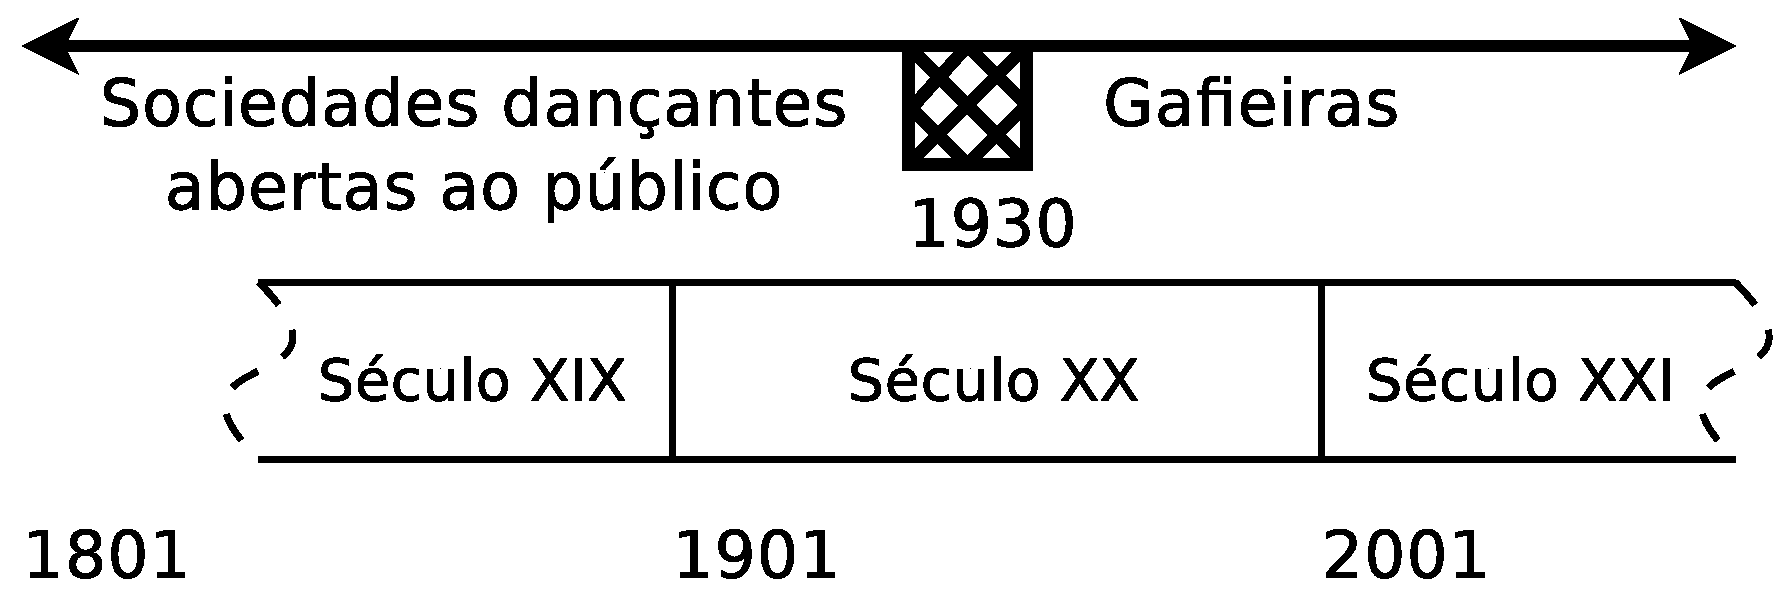
\includegraphics[width=0.65\textwidth]{chapters/cap-intro/gafieira-crono.eps}
  \caption{Cronologia da designação de gafieira para os salões de dança no Rio de Janeiro.}
  \label{fig:gafieiracrono}
\end{figure}

A primeira vez\footnote{Primeira coincidência achada na Biblioteca Digital da Fundação Biblioteca Nacional.} 
que o jornal ``O Radical'' (RJ) usa o neologismo ``gafieira'' 
é o dia 8 de setembro de 1932 \cite[pp. 12]{gafieirajournaloradical1},
com o titular:
\begin{tcolorbox}[breakable,colback=lowgray,colframe=lowgray]%%
A sahida do baile: Por causa de Aracy, o estivador foi ferido á baia.\\
... Na rua Domingo Lopes, n. 243, em Madureira, está situado o club de dança Ideal, 
conhecido pelos moradores locaes por ``Gafieira''.
\end{tcolorbox} 
Ao dia seguinte, 9 de setembro de 1932, o jornal ``A Batalha'' (RJ), 
usava também a palavra ``gafieira'' para se referir ao mesmo incidente \cite[pp. 8]{gafieirajournalabatalha1}.

O ``Jornal do Brasil'', o dia 9 de janeiro de 1934, 
usa também a palavra gafieira \cite[pp. 11]{gafieirajournalbrasil1}, com o titular:
\begin{tcolorbox}[breakable,colback=lowgray,colframe=lowgray]%%
À porta de uma ``gafieira''.
Ainda o conflito da madrugada de domingo no largo de Madureira.
Faleceu um dos soldados no Hospital da Policia Militar. 
Ha no largo de Madureira uma sociedade dansante, mais conhecida por ``gafieira'', 
com entradas retribuidas, ondem de quando em quando, se registram conflitos, 
alguns de graves consequências...
\end{tcolorbox} 
Como é visto nas refecerias dos jornais, 
o termo gafieira, estava associado a lugares um pouco perigosos;
isto propiciado pelo aumento do número de locais que se atribuíam este nome e a diversidade do seu público.
Porem, este não seria o padrão pelo qual se regiam todas as gafieiras, 
e certamente a conotação mais perigosa ou pejorativa iria mudando no tempo. 


Por exemplo, sobre o Elite Club,  nos sabemos que funcionava as quintas, sábados e domingos,
e existia um fiscal no salão (o velho Russo)\cite[pp. 37]{gafieirajournalmanchete}, 
que fazia cumprir estritamente as normas de bom-tom, comportamento social e respeito ao ambiente, como todo clube familiar precisa ter \cite[pp. 12]{respeitojournalbrasil1}; de modo que, 
não eram admitidas damas que não estivessem de sapatos de salto alto \cite[pp. 37]{gafieirajournalmanchete};
homens embriagados não entravam e o traje indispensável era o paletó e gravata, 
ou no mínimo camisa fechada \cite{entrevistajuliojournalbrasil1}.
O cavaleiro não podia abraçar a dama nem sentado na cadeira \cite{entrevistajuliojournalbrasil1},
né dançar de rosto colado, ou por a mão nas costas da dama sem usar lenço \cite[pp. 10]{simoesjournalbrasil1}, 
quem fiscalizava, na porta, era um preto velho tratado por todos de ``titio''  \cite[pp. 37]{gafieirajournalmanchete}.
Se alguma regra não era cumprida, o seu Júlio, jogava a qualquer um para fora \cite{entrevistajuliojournalbrasil1}.
Nos bailes dedicados ao padroeiro, todo 20 de janeiro, era obrigatório vestir de branco,
já seja no traje ou no vestido, incluindo sapatos e camisas \cite[pp. 37]{gafieirajournalmanchete}.
Tão grande era o censo de ordem dos frequentadores do Elite Club, 
que lhe era permitido operar estando a menos de 80 metros de um hospital,
sendo que nessa época existia a Lei n. 1.590 de 1924, 
seguindo a qual nenhuma casa de diversões podia estar a menos de 200 de estabelecimentos hospitalares,
Ate o proprio Delegado Dulcídio Gonçalves, da Delegacia de Costumes,
dispensava-se de mandar policiar o Elite.
``À casa do Júlio não precisa de policiamento'', dizia o Delegado Dulcídio
\cite[pp. 5]{simoesjournalalutademocratica1}.


Assim, ao transcorrer dos anos, essa visão popular mais obscura da palavra gafieira foi mudando;
pelo qual o jornalista Francisco Duarte, o dia 12 de agosto de 1979,
escreve no Jornal no Brasil (RJ) sobre este assunto com o título:
``Gafieira - Tratado geral do ambiente que exige respeito'' \cite{respeitojournalbrasil1},
explicando:
\begin{tcolorbox}[breakable,colback=lowgray,colframe=lowgray]%%
... o verbete Gafieira com o significado de baile reles, arrasta-pé, baile popular de baixa categoria.
No passado, encarada com má vontade pelos puristas do léxico e pela burguesia republicana dançante,
pode ter sido assim. Mas em 1979 -- e cabe aos dicionaristas verificar in loco --
gafieira é baile de clube particular, com entrada paga e freqüência livre, 
local de lazer e dança onde existe bom comportamento e muita compostura,
em perfeita integração racial.\\
(Francisco Duarte)
\end{tcolorbox} 
Além da afirmação anterior, 
o jornalista explica como a ``Delegacia de Diversões Públicas'' classifica as casas de dança;
onde temos: 
\begin{itemize}
\item ``boates'', que são bar restaurantes com pista de dança e palco para show;
\item ``cabarés'', onde se bebe, come, dança e se tem espetáculos de variedades;
\item ``dancings'' onde se dança mediante pagamento em cartões e picotes; e 
\item ``inferninhos'' que são boates de baixa categoria, 
frequentados por pessoas de vida irregular e onde se toca música barulhenta.
\end{itemize} 
Em palavras de Duarte, ``Gafieiras são sinônimos de baile em salão espaçoso como boa música orquestral'' \cite{respeitojournalbrasil1}.



%%%%%%%%%%%%%%%%%%%%%%%%%%%%%%%%%%%%%%%%%%%%%%%%%%%%%%%%%%%%%%%%%%%%%%%%%%%%%%%%
%% SUB SECTION
\subsection{Estatutos da gafieira}\index{Estatuto da Gafieira}
Os "Estatutos da Gafieira" é uma composição musical escrita, por Billy Blanco;
esta foi interpretada por primeira vez na voz de Inezita Barroso, 
numa gravação da "RCA Victor" em janeiro de 1954 \cite{musicaestatuto};
O seguinte texto mostra a letra da música \cite[pp. 95]{musicaestatutojournal1955}.
\begin{tcolorbox}[breakable,colback=lowgray,colframe=lowgray]%%
\center{Moço! Olha o vexame!}\\
O ambiente ``ingige'' respeito!\\
Pelos estatutos da nossa gafieira\\
Dance a noite inteira, mas dance direito!\\
Aliás, pelo artigo 120,\\
O cavalheiro que fizer o seguinte:\\
Subir nas paredes, dançar de pé pro ar,\\
Morar na bebida sem querer pagar,\\
Abusar da umbigada de maneira folgazã,\\
Prejudicando hoje o bom crioulo de amanhã,\\
Será distintamente censurado!\\
Se balançar o corpo, tá na mão do delegado!\\
Balançou o corpo? tá na mão do delegado!\\
\end{tcolorbox}
O texto é uma tentativa bem-humorada do autor de descrever o que acontecia 
nas gafieiras, porem na época da escrita desta popular samba, não
existiam tais estatutos\footnote{Estatutos, no sentido de regulamento, 
ordenança o conjunto de normas legais pelas que se regula o funcionamento de uma corporação ou associação.};
existia um código de costumes sim \cite[pp. 13]{respeitojournalbrasil1} em alguns salões, 
mas cada casa de dança imponia estes no seu local a critério do fiscal do salão ou donos \cite[pp. 10]{simoesjournalbrasil1} \cite{entrevistajuliojournalbrasil1} \cite[pp. 37]{gafieirajournalmanchete},
isto é confirmado por um depoimento realizado por 
Billy Blanco no 8 de julho de 2011 \cite{depoimentobilly}; o texto a seguir
mostra um fragmento dessa entrevista.

\begin{tcolorbox}[breakable,colback=lowgray,colframe=lowgray]%%
"Observando os acontecimentos de uma gafieira, então, eu imaginei
coisas, porque o compositor vive muito da imaginação. E eu criava situações 
possíveis de serem acontecidas na gafieira, ou então narrava o que
acontecia realmente. Por exemplo, no [samba] Pistom de Gafieira, tinha
um cidadão que era pistonista da orquestra que sempre tocava forte para
disfarçar quando a polícia vinha chegando. Doutra feita, eu tive a ideia
de fazer o estatuto para a gafieira. Então eu humorizei, porque ninguém
dança de pé pro ar, nem sobe em parede, não é? Mas a gente cria uma
extravagância dessas para dar uma certa graça, um certo sentido à música.
Na época, não havia código nenhum, eu apenas criei aquilo e muitas gafieiras 
depois tinham esse estatuto na parede para quem quisesse cantar.
Você vê que as regras do estatuto são umas regras brincalhonas, não é?" 
~\\
(Billy Blanco)
\end{tcolorbox}

Mesmo observando que as regras propostas pelo autor tem um caráter humorístico e sarcástico,
o texto foi adotado rapidamente pelas gafieiras, como um chamado a reflexão sobre umas
normas básicas a serem tidas em conta no salão, pois tem um alto grado de bom senso. Por exemplo: 
A linha 7, pode ser interpretada como uma indicação a 
não fazer movimentos aéreos na pista de dança,
ou  evitar movimentos capoerísticos; tudo isto
pelo evidente espacio reduzido e compartilhado que existe na pista de dança, 
além de que os movimentos aéreos estão pensados para ser
executados em apresentações e não em danças sociais. 
A linha 8, nos lembra o respeito ao parceiro; pois a pessoa que dança precisa
estar no controle de suas faculdades físicas e mentais; 
no caso dos condutores\footnote{\label{footlab:conducao}Nas danças sociais é comumente usado o paradigma da condução; 
onde no casal, uma pessoa assume o papel de condutor dos movimentos e 
a outra pessoa assume o papel de seguidor, este recebe a informação da condução e retorna uma resposta corporal.}, 
para estar atentos ao salão e cuidar do seu par enquanto os movimentos são executados, 
e no caso do seguidor\footref{footlab:conducao} para evitar problemas
nos giros e outros movimentos que precisem  controle do eixo do corpo.
As linhas 9 e 10 indicam sobre um conjunto de expressões artísticas 
afro-brasileiras emolduradas no século XIX com o nome de "samba umbigada" \cite[pp. 47]{diniz2008almanaque} \cite[pp. 85]{sandroni2001feitico}; nestas danças existe
um movimento chamado "umbigada" \cite{da2015historia} que da nome à dança, onde o ventre do homem e da mulher batem geralmente para indicar
a troca de dançarino; assim as linhas 9 e 10 se referem a
 evitar "abusar" de movimentos de umbigada que provem de danças que não eram bem vistas na época e eram consideradas gentílicas \cite[pp. 85]{sandroni2001feitico}.
Finalmente,
a linha 12 fala sobre balançar o corpo, que seguindo o contexto cultural, 
pode indicar não agir como bêbado\footnote{``Balançar o corpo; agitar, como o bebado, mal firme, e outros táes''-Diccionario da lingua portugueza, 1858.} \cite[pp.296]{diccionario1858}, ou em outras palavras,
com pouca elegância ou respeito,
caso contrario seria levado à delegacia!.



%%%%%%%%%%%%%%%%%%%%%%%%%%%%%%%%%%%%%%%%%%%%%%%%%%%%%%%%%%%%%%%%%%%%%%%%%%%%%%%%
%% SECTION
%%%%%%%%%%%%%%%%%%%%%%%%%%%%%%%%%%%%%%%%%%%%%%%%%%%%%%%%%%%%%%%%%%%%%%%%%%%%%%%%
\section{Historia da música do samba}\index{música do samba}



\textcolor{red}{Pelo telefone}



%%%%%%%%%%%%%%%%%%%%%%%%%%%%%%%%%%%%%%%%%%%%%%%%%%%%%%%%%%%%%%%%%%%%%%%%%%%%%%%%
%% SECTION
%%%%%%%%%%%%%%%%%%%%%%%%%%%%%%%%%%%%%%%%%%%%%%%%%%%%%%%%%%%%%%%%%%%%%%%%%%%%%%%%
\section{Historia da samba de gafieira}\index{historia da samba de gafieira}


O aparecimento do samba, 
foi um grande impacto para as pessoas que frequentavam estes já existosos lugares de dança;
sendo considerado um ritmo novo e ligeiro,
que desagradou aos bailarinos de maior idade e menos ágeis \cite[pp. 3]{entrevistajuliojournalbrasil1}.
O senhor, Júlio Simões chegou a temer pelo futuro da ``Kananga do Japão'' e
do ``Elite Club''; porem, para sorte dele, 
o samba fez muito sucesso no Elite,
e passou a ser considerado matéria indispensável para qualquer pessoa que pretendesse ser bailarino, 
compositor ou instrumentista \cite[pp. 3]{entrevistajuliojournalbrasil1}.

\textcolor{red}{Historia
\begin{description}
\item [A] Perna, Marco Antonio (2001). Samba de Gafieira - a história da dança de salão brasileira. ISBN 85-901965-5-0
\end{description}
}





\chapterimage{chapter_head_2.pdf} % Chapter heading image

\chapter{\textcolor{green}{Regras na dança de salão}}

\index{Regra} 
\begin{definition}[Regra:]
Norma, lei, costume que dirige, orienta e regula procedimentos (regra gramatical; regras de etiqueta; regras na dança).
[http://www.aulete.com.br/regra]
\end{definition}
\index{Condução} 
\begin{definition}[Paradigma da condução (Dança):] Este é usado na dança de salão, 
e implica que na dança a dois existe uma transmissão de informação
entre as pessoas que conformam o casal, 
de modo que a informação/comando tem um fluxo unidirecional no médio de transmissão,
que vá desde o condutor ate o seguidor. 
\end{definition}
\index{Condutor} 
\begin{definition}[Condutor (Dança):] 
A pessoa que tem o papel de conduzir e propor o movimento. 
O objetivo técnico das pessoas que optam por este rol é chegar 
a ter o sensibilidade necessária para entender onde está localizado espacialmente, 
e como distribui o peso do corpo, o seguidor; 
de modo que seja possível para o condutor aplicar uma mistura de forças e torções sobre o seguidor para provocar o movimento desejado;
chama-se a isto saber conduzir.
Sinônimos de condutor: Líder.
\end{definition}
\index{Seguidor} 
\begin{definition}[Seguidor (Dança):] 
A pessoa que recebe a condução e proporciona uma resposta corporal. 
O objetivo técnico das pessoas que optam por este rol é chegar 
a ter a sensibilidade necessária para entender as conduções,
independentemente de quem seja a pessoa que aplique a condução;
chama-se a isto ser conduzível.
Sinônimos de seguidor: Conduzido.
\end{definition}
\index{Dança social} 
\begin{definition}[Dança social:]
É uma dança com fim recreativo de prática social, não cênica, nem competitiva, 
que não tem um interesse artístico, histórico, geográfico ou técnico; 
que se universaliza e consiste em movimentos dos corpos de um casal, 
onde existe a figura condutor e o seguidor (papeis intercambiáveis) \cite{Zamoner2012} ate onde o nível técnico do par o permita.
\end{definition}
\index{Dança de salão} 
\begin{definition}[Dança de salão:]
É uma arte que procura conservar suas características técnicas, 
sua origem histórica e geográfica, e se universaliza em práticas sociais. 
Esta arte consiste na interpretação improvisada da música por médio dos movimentos 
dos corpos de um casal, utilizando um paradigma da dança onde se tem um condutor e um seguidor (papeis intercambiáveis) \cite{Zamoner2012}.
\end{definition}

Neste capítulo veremos um conjunto de regras, e a explicação de como o cumprimento
ou não destas afetam ao desenvolvimento estético e técnico da dança de 
salão\footnote{Ou na dança social sim se interessa levar estas ideias a esse âmbito.}  no paradigma da condução.

Assim, serão usados neste capítulo termos como "condutor" e "seguidor", 
mas isto não implica nenhuma obrigatoriedade ou restrição, das pessoas, para o uso de algum destes papéis na dança;
porem é comum ver que o papel de condutor é escolhido tradicionalmente pelos "cavalheiros" e o papel de seguidor pelas "damas".
%só são um recurso literário para o melhor entendimento das explicações mostradas aqui.
\begin{lattention}
É importante aclarar
que as regras expostas neste capítulo não estão regulamentadas por nenhuma entidade ou intituição; assim, estas
refletem, o meu aprendizado de distintos professores,
interpretações pessoais  e deduções. 
\end{lattention}

%%%%%%%%%%%%%%%%%%%%%%%%%%%%%%%%%%%%%%%%%%%%%%%%%%%%%%%%%%%%%%%%%%%%%%%%%%%%%%%%
\section{\textcolor{green}{Regras gerais na dança de salão}}
As regras que veremos aqui abrangem um conjunto amplo de estilos de 
dança, e não devem ser
tratadas como leis, e sim como diretrizes a serem usadas como padrão de inicialização, de modo que 
o dançarino ou dançarina analisará cada caso e se necessário criará uma exceção e atuará conforme ela.
A continuação são listadas algumas regras gerais na dança de salão.\\

\begin{itemize}
\item \textbf{Rodar o salão:} Que os dançarinos executem sua dança girando o salão, 
é importante para criar a ilusão de que o espaço de dança é maior, dado que mesmo
tendo uma pista de dança lotada, o espaço que um
casal deixa ao se movimentar é ocupado pelo casal que vem atrás deles, criando 
assim um fluxo de movimento circular que permite a todos os casais usar a pista de dança
na sua totalidade (por convenção o sentido de giro é sempre anti-horário); 
visto o anterior é importante ressaltar que né todas as danças tem
uma evolução circular na pista de dança, pois existem estilos de dança que são dançados em linha,
como por exemplo a "Salsa em linha" ou o "West coast swing", ou também existem estilos que
tem um comportamento hibrido entre circular e linha como o "Zouk". Neste sentido,
a "samba de gafieira"  tem um comportamento circular e se deveria dançar
rodando o salão para um boa etiqueta na pista de dança.
\item \textbf{Conduzir e ser conduzidos:} Trabalhar num paradigma da dança baseado
na condução é muito importante para as danças de salão, dado que isto implicará
que um condutor habilidoso poderá dançar fluidamente com pessoas com quem nunca dançou
antes (se esta for conduzível). O mesmo acontecerá para as pessoas que desenvolvam
a sensibilidade necessária para serem conduzíveis, elas poderão dançar com qualquer
condutor, inclusive poderão ter um desenvolvimento básico em estilos de dança pouco ou não conhecidos.
O caso contrario ao paradigma da condução, é ter um estilo de dança baseado em coreografias;
este enfoque, dependendo da finalidade, pode ser visto como um vicio que geralmente aparece quando iniciamos
na dança. Isto acontece, no caso do condutor, quando este assume que se realiza a parte do movimento 
que lhe corresponde (na parte visual) sem enviar nenhuma informação ao seguidor, 
este tem que reconhecer/adivinhar o movimento, e realizar a parte que lhe corresponda. Este enfoque
funciona bem quando ambos tem treinado antecipadamente os movimentos, e/ou conhecem a sequencia
em que estes movimentos serão executados, porem falha quando os dançarinos não se conhecem;
comprovar isto é fácil se imaginamos por exemplo o caso em que o condutor executa um movimento
que tem a parte inicial muito parecida a outro movimento, neste caso, se o seguidor não tiver
um poder telepático confundirá um movimento com o outro e acontecerá um problema de comunicação. Assim, a coreografia
na dança deve estar reservada para apresentações, onde o casal volta 
a sua atenção para a encenação da peça, e não para detalhes mais mecânicos.

\item \textbf{Ter o peso do corpo sobre um pé só no final da proposta de movimento:} 
Na dança de salão é muito importante a leveza e o auto controle mostrado na 
execução dos movimentos; assim, para conseguir isto, é importante que os dançarinos
tenham o peso do corpo num pé só ao terminar a execução de cada movimento; o motivo
é facilmente percebido se fazemos um pequeno exercício. Ao ficar em pé separamos as
pernas uma distancia igual à de nosso quadril, e nesse momento levamos o peso do corpo
(concentrado no nosso centro de gravidade que nesse casso está perto do umbigo) a
apontar a um ponto médio entre nossos pés, nesse instante estamos dividindo o peso do corpo
entre nossos pontos de apoio, 50$\%$ no pé direito e 50$\%$ no pé esquerdo; agora, mantendo o peso
do corpo nesse lugar, tentaremos levantar qualquer de nossos pés, será evidente
que esse trabalho é muito difícil sem perder o equilíbrio, pois para mantê-lo
precisamos de ambos pontos de apoio; casos similares podem ser vistos com qualquer proporção de distribuição de peso,
por exemplo, 30$\%$ e 70$\%$ ou 20$\%$ e 80$\%$. Assim o único caso em que estamos
equilibrados e podemos executar nosso movimento e levantar um pé 
mantendo a postura e auto controle, é quando
temos o 100$\%$ do peso do corpo num pé só, o pé de apoio. 
Por outro lado, quando consideramos ao condutor como o agente desequilibrante do seguidor, por exemplo no caso
em que este aplica uma condução;
a regra de manter o peso do corpo num pé só, tem um valor agregado; 
pois fica mais fácil para o condutor orientar
ao seguidor a fazer o seguinte movimento, dado que o único pé que este pode mover é o pé
que está livre, e que é o pé que o condutor precisa que se movimente, 
além de que a força necessária pelo condutor para tirar ao seguidor do seu equilíbrio 
atual é muito menor ao caso quando o seguidor tem dois pontos de apoio.
Adicionalmente o seguidor tem um pé livre para se resguardar do desequilíbrio provocado pelo 
condutor e adquirir um novo equilíbrio com esse pé.

\item \textbf{Ter uma abraço de dança firme:} Seguindo a ideia da condução, esta só pode
ser realizada se existe um médio de comunicação, onde possa ser transmitido
o comando do condutor ao seguidor. Assim, um bom abraço garante este
fluxo de informação.
\end{itemize}

%%%%%%%%%%%%%%%%%%%%%%%%%%%%%%%%%%%%%%%%%%%%%%%%%%%%%%%%%%%%%%%%%%%%%%%%%%%%%%%%
\section{\textcolor{blue}{Regras gerais na samba de gafieira}}


\begin{itemize}
\item \textbf{Quadril avança, ombros e pé acompanham}  O movimento inicia no quadril.
\item \textbf{Quando movimentar um pé chegar com 100$\%$ do peso do corpo} estética da samba de gafieira.
\item \textbf{Braços firmes do seguidor} estes transportam a informação para o quadril (ex: picadilho).
\item \textbf{Abraço uniforme do condutor} este procura manter a mesma distancia (ex: gancho redondo).
\item \textbf{O tórax do condutor guia ao seguidor} O tórax do condutor guia ao seguidor (NÃO o braço).
\item \textbf{Procurar o paralelismo de ombros e linha de visão do casal} é responsabilidade do seguidor seguir ao condutor, indução.
\item \textbf{O pé de apoio debe estar apontando a um ponto médio entre os pês do par de dança} .
\end{itemize}


\chapterimage{chapter_head_2.pdf} % Chapter heading image

\chapter{Fundamentos de notação musical}
Nas seguintes sub seções abordaremos os termos compasso, tempo e contratempo,
num sentido rítmico (distribuição de tempos) e não explicaremos o significado 
melódico (distribuição de frequências) das 
figuras musicais na partitura, devido a que as explicações mostradas aqui estão
orientadas para um público interessado na dança, que precisa numa primeira 
aproximação à música, conhecer rapidamente a parte rítmica dela. Para aprofundar mais na parte 
melódica recomendamos acudir a materiais, livros ou revistas especializadas \cite{medteoria}
\cite{azevedocompor} \cite{alves2004teoria} \cite{mascarenhascurso} \cite{adolfo2002musica} \cite{grabner2001teoria}.
%%%%%%%%%%%%%%%%%%%%%%%%%%%%%%%%%%%%%%%%%%%%%%%%%%%%%%%%%%%%%%%%%%%%%%%%%%%%%%%%
\section{Compasso}
\label{sec:compaso}

O dicionário de Harvard de música \cite{randel2003harvard} define compasso (``meter'' em inglês)
como: ``O padrão em que uma sucessão constante de pulsos rítmicos é organizada'', também indica que
``o compasso de uma obra ou uma porção dela é indicado geralmente por uma fração'', como por exemplo:
${2}/{2}$ , ${3}/{4}$ , ${4}/{4}$, etc; em português é chamada a esta fração como a formula do compasso. 

 
O denominador da formula do compasso indica o valor da pulsação básica (tempo) do padrão de repetição (compasso), 
e o numerador indica o número dessas pulsações que compõem o compasso. Assim, com a ajuda da
Tabela \ref{tab:noteslength}; onde a primeira coluna mostra a formula do compasso (só o denominador),
a segunda coluna mostra as figuras musicais que o denominador da formula evoca, e a terceira e
quarta coluna, representam a duração em segundos e o nome da figura musical;
podemos achar equivalências aos exemplos da formula do compasso dados
anteriormente; onde os compassos com formula $\mathbf{2}/2$ tem cada um, uma duração de $\mathbf{2}$\halfnote ~(duas mínimas),  
compassos com formula $\mathbf{3}/4$ tem uma duração de $\mathbf{3}$\quarternote ~(trés semínimas) 
e $\mathbf{4}/4$ uma duração de $\mathbf{4}$\quarternote ~(quatro semínimas). É importante
ressaltar que a duração em tempo das figuras musicais é relativa, como pode ser visto
na terceira coluna da Tabela \ref{tab:noteslength}, onde as durações estão em função
da duração $S$ da semibreve. 
\begin{table}[h]
\centering
\begin{tabular}{|c|c|c|c|}
\hline
formula & Figura  & Duração & Nome\\ \hline
\hline
$1/1$   & \fullnote    & $S$   & Semibreve \\ \hline
$1/2$ & \halfnote    & $S/2$ & Mínima \\ \hline
$1/4$ & \quarternote & $S/4$ & Semínima \\ \hline
$1/8$ & \eighthnote  & $S/8$ & Colcheia \\ \hline
\end{tabular}
\caption{Duração e símbolos de algumas figuras musicais}
\label{tab:noteslength}
\end{table}

Se classificamos aos compassos por sua métrica, os três tipos mais conhecidos 
são os compassos binários, ternários, quaternários \cite[pp. 27]{adolfo2002musica}.

\textbf{Um compasso binário} é uma estrutura rítmica que se carateriza por ter compassos com dois tempos,
sendo o primeiro pulso forte e o segundo fraco \cite[pp. 66]{adolfo2002musica}\cite[pp. 28]{alves2004teoria}. Em geral podem ser chamados
de compassos binários quando a formula de compasso tem a forma $2A/B$, 
onde $A$ pode ser $1$ ou $3$ e $B$ pode ser $2$, $4$, $8$, etc.
Por exemplo as formulas: $2/8$, $2/4$, $2/2$,  $6/16$, $6/8$ e  $6/4$;
representam compassos binários.
Alguns autores consideram aos compassos quaternários (ex: 4/4, 12/4) como um caso de compasso binário,
chamando eles de compasso binário duplo \cite[pp. 41]{grabner2001teoria}.
A Figura \ref{compasso:binario}, representa um exemplo de compasso binário, com 
formula de compasso $2/2 \equiv 2$\halfnote, onde o primeiro e segundo
compasso tem uma duração de $S$ (uma semibreve), o primeiro compasso contem $2$\halfnote~e
o segundo contem $4$\quarternote.
\begin{figure}[H]
\centering
\begin{abc}[name=compasso1]
X: 1 % start of header
K: C % scale: C major
M: 2/2 %meter - compasso
"Primeiro compasso" G4 F4 |"Segundo compasso" G2 D2 F2 D2  |
\end{abc}
\caption{Exemplo de compasso binário}
\label{compasso:binario}
\end{figure}

\textbf{Um compasso ternário} 
é uma estrutura rítmica que se carateriza por ter compassos com trés tempos,
sendo o primeiro pulso forte e os outros dois fracos 
\cite[pp. 67]{adolfo2002musica}\cite[pp. 30]{alves2004teoria}. Em geral podem ser chamados
de compassos ternários quando a formula de compasso tem a forma $3^A/B$, 
onde $A$ pode ser $1$ ou $2$ e $B$ pode ser $2$, $4$, $8$, etc.
Por exemplo as formulas: $3/8$, $3/4$, $3/2$,  $9/16$, $9/8$ e $9/4$;
representam compassos ternários (com denominador múltiplo de 3 exclusivamente) 
A Figura \ref{compasso:ternario}, representa um exemplo de compasso ternário, com 
formula de compasso $3/4 \equiv 3$\quarternote, onde o primeiro e segundo
compasso tem uma duração de $0.75S$, o primeiro compasso contem $3$\quarternote~e
o segundo contem $6$\eighthnote.
\begin{figure}[H]
\centering
\begin{abc}[name=compasso2]
X: 1 % start of header
K: C % scale: C major
M: 3/4 %meter - compasso
"Primeiro compasso" G2 F2 F2 |"Segundo compasso" G1 F1 E1 D1 D1  D1  |
\end{abc}
\caption{Exemplo de compasso ternário}
\label{compasso:ternario}
\end{figure}


\textbf{Um compasso quaternário}  
é uma estrutura rítmica que se carateriza por ter compassos com quatro tempos,
sendo o primeiro pulso forte o segundo fraco o terceiro semiforte e o ultimo fraco 
\cite[pp. 67]{adolfo2002musica}\cite[pp. 32]{alves2004teoria}. 
Em geral podem ser chamados
de compassos quaternários quando a formula de compasso tem a forma $4A/B$, 
onde $A$ pode ser $1$ ou $3$ e $B$ pode ser $2$, $4$, $8$, etc.
Por exemplo as formulas: $4/8$, $4/4$, $4/2$,  $12/16$, $12/8$ e $12/4$;
representam compassos quaternários 
A Figura \ref{compasso:quaternario}, representa um exemplo de compassos quaternário, com 
formula de compasso $4/4 \equiv 4$\quarternote, onde o primeiro e segundo
compasso tem uma duração de $S$, o primeiro compasso contem $4$\quarternote~e
o segundo contem $8$\eighthnote.
\begin{figure}[H]
\centering
\begin{abc}[name=compasso3]
X: 1 % start of header
K: C % scale: C major
M: 4/4 %meter - compasso
"Primeiro compasso" G2 D2 F2 D2|"Segundo compasso" G1 F1 D1 C1 F1 E1 D1 C1 |
\end{abc}
\caption{Exemplo de compasso quaternário}
\label{compasso:quaternario}
\end{figure}


%%%%%%%%%%%%%%%%%%%%%%%%%%%%%%%%%%%%%%%%%%%%%%%%%%%%%%%%%%%%%%%%%%%%%%%%%%%%%%%%
\section{Tempo}

Como já foi sugerido na Seção \ref{sec:compaso}, é chamado de "tempo" 
à pulsação básica e unidade de medida dos compassos nas composições musicais;
assim, temos que compassos binários, ternários e quaternários tem uma duração 2 tempos, 
3 tempos e 4 tempos, respetivamente. Por comodidade chamaremos $T$ à duração em segundos de cada tempo,
sendo que o valor de $T$ variará dependendo da formula de compasso usada.


É importante
ressaltar que os compassos que usem a mesma formula de compasso terão sempre a mesma duração em segundos;
por outro lado, podem ser achados casos onde compassos com diferente formula podem ter a mesma duração;
por exemplo: compassos binários com formula $\mathbf{2}/2$, como na Figura \ref{fig:tempo1}, 
\begin{figure}[H]
\centering
\begin{abc}[name=tempo1]
X: 1 % start of header
K: C % scale: C major
M: 2/2 %meter - compasso
G2 D2 F2 D2 | G4 F4 |
w: T/2 T/2 T/2 T/2  Tempo Tempo
\end{abc}
\caption{Exemplo de dois compassos com 2 tempos de duração T}
\label{fig:tempo1}
\end{figure}
terão uma duração de dois tempos ($2T$) \cite[pp. 25]{azevedocompor} onde cada tempo ($T$) tem uma duração 
de uma mínima (\halfnote), ver Tabela \ref{tab:noteslength}.

Por outro lado,
compassos quaternários com formula $\mathbf{4}/4$, como na Figura \ref{fig:tempo2}, 
\begin{figure}[H]
\centering
\begin{abc}[name=tempo2]
X: 1 % start of header
K: C % scale: C major
M: 4/4 %meter - compasso
G2 D2 F2 D2| G4 F4|
w: Tempo Tempo Tempo Tempo 2T 2T
\end{abc}
\caption{Exemplo de dois compassos com 4 tempos de duração T}
\label{fig:tempo2}
\end{figure} 
terão uma duração de 4 tempos ($4T$) \cite[pp. 25]{azevedocompor} onde 
cada tempo ($T$) tem uma duração de uma semínima (\quarternote), ver Tabela \ref{tab:noteslength}.
Assim, estas duas formulas ($2/2$ e $4/4$) representam compassos 
com a mesma duração em segundos, uma semibreve (\fullnote),
porem tem valores diferentes para a variável $T$ em segundos.

\begin{lattention}
Se interpretamos a música mostrada nas Figuras \ref{fig:tempo1} e \ref{fig:tempo2},
podemos perceber que ambas descrevem um sonido similar; assim, não é fácil
distinguir só escutando se o sonido provem de um compasso com formula $2/2$ ou $4/4$.
Em estos casos e similares o mais factível é afirmar que pertencem a alguma sub categoria da família dos
compassos binários, seguindo o critério de alguns autores \cite[pp. 41]{grabner2001teoria} que afirmam 
 que os compassos
quaternários são uma sub categoria de compassos binários.
\end{lattention}

%%%%%%%%%%%%%%%%%%%%%%%%%%%%%%%%%%%%%%%%%%%%%%%%%%%%%%%%%%%%%%%%%%%%%%%%%%%%%%%%
\section{Contratempo}
Um contratempo acontece quando as notas (representadas por figuras musicais na partitura) 
são executadas em tempos fracos do compasso
ou nas partes fracas dos tempos, sendo que estas estão intercaladas por pausas nos tempos
fortes ou partes fortes dos tempos \cite[pp. 16]{mascarenhascurso} 
\cite[pp. 36]{azevedocompor}, neste sentido o contratempo pode ser visto como a 
omissão de notas nos tempos fortes ou nas partes fortes dos tempos \cite[pp. 146]{medteoria}.
Ou ``num sentido mais amplo, o contratempo é a acentuação de um tempo fraco em vez de um tempo forte'' \cite[pp. 147]{medteoria}. 

Assim é fácil de perceber que a palavra ``contratempo'' na música, 
é um adjetivo que faz referencia a como estão configuradas ou acentuadas 
as notas no compasso. Por exemplo:
A Figura \ref{fig:contratempoa} mostra 
quatro compassos (binários) com formula $2/4$, em cada compasso existem 
contratempos nos tempos fracos ou nas partes fracas dos tempos, sendo que cada tempo
tem uma duração de uma semínima (\quarternote) e cada compasso uma duração 
de uma mínima (\halfnote), ou seja duas semínimas (2\quarternote). 
\begin{itemize}
\item ``F''  indica que é o tempo é forte, 
\item ``f''  indica que é o tempo é fraco,
\item ``FF'' indica que é a parte forte de um tempo forte,
\item ``Ff'' indica que é a parte fraca de um tempo forte,
\item ``fF'' indica que é a parte forte de um tempo fraco,
\item ``ff'' indica que é a parte fraca de um tempo fraco, 
\end{itemize} 

finalmente
a figura musical \ViPa~ indica um silencio da mesma duração que uma semínima (\quarternote)
e a figura musical \AcPa~ indica um silencio da mesma duração que uma colcheia (\eighthnote).
\begin{figure}[H]
\centering
\begin{abc}[name=contratempoa]
X: 1 % start of header
K: C % scale: C major
M:2/4
%T: Contratempo num compasso binário
V:1 clef=treble name="A" sname="A"
[V:1] "F"z2 "f"G2 | "FF"z1 "Ff"G1  "fF"z1 "ff"G1 | "FF"z1 "Ff"G1  "f"G2 |  "F"z2 "fF"z1 "ff"G1  |
w:          Tempo          T/2            T/2             T/2     Tempo                 T/2
\end{abc}
\caption{Contratempos no tempos fracos ou nas partes fracas dos tempos}
\label{fig:contratempoa}
\end{figure}
Na Figura \ref{fig:contratempoa}, existem contratempos em todos os compassos porem estes estão
configurados de distintas formas;
no primeiro compasso acontece um contratempo dado que a única nota é executada 
no tempo fraco do compasso, no segundo compasso acontecem contratempos pois as 
notas são executadas nas partes fracas de cada tempo,
no terceiro compasso acontece um contratempo pela execução de uma nota na parte 
fraca do tempo forte, sendo o resto do tempo preenchido com um silencio, e 
finalmente no quarto compasso acontece um contratempo pela execução de uma nota
na parte fraca do tempo fraco, sendo o resto do compasso preenchido com silêncios.


Por outro, A Figura \ref{fig:contratempob} mostra como o contratempo pode ser 
expressado como a acentuação de um tempo fraco em vez de um tempo forte \cite[pp. 147]{medteoria}. 
\begin{figure}[H]
\centering
\begin{abc}[name=contratempob]
X: 1 % start of header
K: C % scale: C major
M:2/4
%T: Contratempo num compasso binário
V:1 clef=treble name="A" sname="A"
[V:1] "F"G2 "f"+accent+G2 | "FF"G1 "Ff"+accent+G1  "fF"G1 "ff"+accent+G1 | "FF"G1 "Ff"+accent+G1  "f"G2  | 
w:    Tempo Tempo           T/2    T/2             T/2    T/2              T/2    T/2             Tempo   
\end{abc}
\caption{Contratempos pela acentuação dos tempos fracos ou nas partes fracas dos tempos}
\label{fig:contratempob}
\end{figure}

%%%%%%%%%%%%%%%%%%%%%%%%%%%%%%%%%%%%%%%%%%%%%%%%%%%%%%%%%%%%%%%%%%%%%%%%%%%%%%%%
\section{Contagem dos tempos musicais desde o ponto de vista do ouvinte}
Antes de iniciar esta seção é importante mencionar uma
problemática que é vista com muita frequência nas escolas de dança; esta é gerada devido a que: A forma em que os tempos são contados 
nos compassos, é
diferente à realizada entre profissionais da música e da dança. 
Sendo que a contagem dos profissionais da música segue as normas
e notações indicadas na partitura, e no caso de profissionais da dança segue geralmente um enfoque 
particular a cada escola de dança, visando só em muitos casos o fácil entendimento do aluno da
execução dos movimentos, e não uma rigorosidade teórica no uso de termos e 
expressões musicais.

Conhecido Tudo isto,
quando escutamos uma música na qual é tipicamente dançado samba de gafieira,
podemos distinguir que a soma dos sonidos produzidos pelos instrumentos realizam 
um padrão de repetição muito particular, geralmente ligado à onomatopeia ``Chic Chic Tum''.
Este padrão está constituído de dois sons ``Chic'' da mesma duração em segundos, 
e um sonido ``Tum'' que ocupa o mesmo tempo que a duração de dois ``Chic''.


A Figura \ref{fig:caquarela} representa os compassos 18, 19 e 20 da  
composição musical ``Aquarela do Brasil'' escrita
por Ary Barroso em 1939 \cite{AquarelaDoBrasil}; 
a versão mostrada na figura teve arranjos por Irineu Krüger \cite{Irineu}. 
Nesta versão, a música está representada com 1 voz ou coro de voces (``Voice Choir'') e 4 
instrumentos (``Eb'',``Bb'',``Strings'' e ``D. Bass''), que usam uma 
formula de compasso $2/4$, de modo que cada compasso
é binário e
pode ser preenchido usando duas semínimas (2\quarternote).

\begin{figure}[H]
\centering
%\includegraphics[width=\textwidth]{chapters/cap-fundamentos/aquarela.png}
\begin{abc}[name=caquarela]
% abcm2ps aquarela.abc  -O aquarela.ps
% ps2epsi aquarela.ps aquarela.eps
%
X: 1 % start of header
T: Brazil - Aquarela do Brasil
C: Music: Ary Barroso, 1939
C: Arranged by: Irineu Krüger
K: C % scale: C major
M: 2/4 % formula do compasso
%
V:1 clef=treble name="Voice Choir" sname="Voice Choir"
V:2 clef=treble name="Eb" sname="Eb"
V:3 clef=treble name="Bb" sname="Bb"
V:4 clef=treble name="Strings" sname="Strings"
V:5 clef=bass   name="D. Bass" sname=""D. Bass"
%
%
[V:1] "18" C'3/2A/2C2  |"19" A3/2(G/2 G/2)E1E/2  |"20" z/2 C'1A/2 C'1C'1  |
w:    Ó Bras-sil        sam-ba_ que dá       bam-bo-leio_ 
w:    Ó Bras-sil        ver-de que dá_       pa-ra~o mun-do 
%
%
[V:2] G1z/2G1z/2G1  | G1z/2G1z/2G1  | G1z/2G1z/2G1  |
%
%
[V:3] z4  | z4  | z4  |
%
%
[V:4] G1z/2G1z/2G1  | G1z/2G1z/2G1  | G1z/2G1z/2G1  |
%
%
[V:5] C,2 G,,2  | C,1 z1 G,,2  | C,2 G,,2  |
\end{abc}
\caption{3 compassos da partitura da composição ``Aquarela do brasil''}
\label{fig:caquarela}
\end{figure}
Analisando esta partitura \cite{Irineu} e escutando a música produzida, podemos perceber facilmente
que os instrumentos executados geram um sonido
com a onomatopeia ``e Chic Chic Tum'' ou ``Chic Chic Tum'' dependendo da percepção do ouvinte. 
Assim, como pode ser escutado, o inicio de cada compasso coincide com o ``Tum''; 
sendo que este é o momento em que a maioria dos instrumentos produzem um sonido, de modo que a sensação para o 
ouvinte é de uma potencia de som maior. Cada instrumento prolongará seu sonido de
forma diferente, porem na percepção final podemos dizer que: o ``Tum'' ocupa 1 
tempo (\quarternote) se conseguimos escutar  ``Chic Chic Tum'' (ver ``D. Bass''), ou 0.75 de tempo se escutamos
``e Chic Chic Tum''. Imediatamente depois do ``Tum'', a 0.75 do primeiro tempo do compasso,
na parte fraca do tempo fraco, 
acontece um sonido com onomatopeia ``e'' que se prolonga incluindo a parte forte do tempo fraco, 
este sonido é executado pelos instrumentos ``Eb'' e ``Strings'' constituindo assim uma sincopa \cite[pp. 143]{medteoria}.
%%Esta é uma sincopa
O segundo tempo (tempo fraco) inicía com o instrumento ``D. Bass'' que produz o primeiro ``Chic''
e finalmente os instrumentos ``Eb'' e ``Strings'' executam o segundo ``Chic''
na parte fraca do tempo fraco, preenchendo o resto do tempo com silêncios, é dizer
fazem contratempos.

Pelo exposto anteriormente, agora podemos simplificar a partitura para gerar um sonido com onomatopeia
``Chic Chic Tum'', como é mostrado na Figura \ref{fig:contratempo1}.
Assim,
o instrumento 1 executa dois sonidos, de modo que o primeiro contribui ao sonido 
``Tum'' e o segundo sonido gera o segundo ``Chic'' do compasso; por outro lado,
o instrumento 2 executa um ritmo com um padrão
de repetição de dois sonidos ``Tum'' e ``Chic'', nesse ordem;
sendo que a nota executada no tempo forte produz um sonido mais agudo que a 
executada no tempo fraco.
\begin{figure}[H]
\centering
\begin{abc}[name=contratempo1]
X: 1 % start of header
K: C % scale: C major
M:2/4
%T: Contratempo num compasso binário
V:1 clef=treble name="Instrumento 1" sname="Inst. 1"
V:2 clef=bass   name="Instrumento 2" sname="Inst. 2"
[V:1] " ""T/2"G1 " ""T/2"z1 " ""T/2"z1 " ""T/2"G1 | " ""T/2"G1 " ""T/2"z1 " ""T/2"z1 " ""T/2"G1  :|
w:    Tum                     Chic                  Tum                   Chic           
[V:2] "Tempo"C,2 "Tempo"G,,2  | "Tempo"C,2 "Tempo"G,,2  :|
w:    Tum       Chic         Tum       Chic            
\end{abc}
\caption{Padrão de repetição para gerar um sonido de onomatopeia ``Chic Chic Tum''.}
\label{fig:contratempo1}
\end{figure}

Pelo exposto anteriormente é fácil perceber, como existe uma diference entre 
o que percebemos ao escutar uma música e a forma como esta é escrita na partitura;
pois como é visto na Figura \ref{fig:contratempo1}, quando escrevemos
um sonido com o padrão de repetição ``Tum Chic Chic'', para o ouvinte é mais natural associar
este sonido com o padrão ``Chic Chic Tum'', devido a que \textbf{ao falar o ser humano usa a pausa
para denotar o final de uma palavra}, da mesma forma, ao escutar uma música, traduzimos
que o sonido que tem um silencio maior apos ser executado marca o final do ciclo
do padrão de repetição. Assim, o que um músico vê ao ler uma partitura
é um padrão de repetição ``Tum Chic Chic'', sendo que  um
ouvinte interpretará de forma instintiva que o padrão é ``Chic Chic Tum ''.

Esta diferença na contagem leva a um problema, sim se quer ser rigoroso na 
forma de contar os tempos nos compassos; por exemplo, na Tabela \ref{tab:ritmo1} 
podemos ver 4 formas distintas de contar os tempos nos compassos indicando a 
distribuição de tempos, onde ``A'' representa uma porção de tempo.
\begin{table}[ht]
  \centering
  \begin{tabular}    {c|ccc|c}
    \hline
    Tipos de contagem       & A/2 & A/2   & A & Recomendável?\\
    \hline
    Contagem 1: & Chic  & Chic  & Tum   & Sim\\
    Contagem 2: & Con   & -tra  & Tempo & Não\\
    Contagem 3: & 1     & e     & 2     & Não\\
    Contagem 4: & 1     & 2     & 3     & Não\\
    \hline
  \end{tabular}
  \caption{Tipos de contagem na samba de gafieira.}
\label{tab:ritmo1}
\end{table}
A contagem 1 é a que recomendo, devido a que pode ser usada sem aprofundar demasiado 
na notação musical, de modo que só precisa ser explicado que a duração de um 
``Tum'' é o dobro que um ``Chic'', e anexado que geralmente veremos que o ``Tum''
acontece no tempo 1 da música, de modo que outra contagem valida seria ``Tum Chic Chic''; 
porem a contagem 1 não está restrita ao uso destas silabas (``Chic'' e ``Tum''), em geral esta
contagem representa a quase qualquer padrão de repetição
que use duas silabas diferentes como os padrões: ``Ta Ta Kum'', ``Tic Tic Pa'', etc. Sendo
que o padrão que não recomendo é o visto na contagem 2 (``Con-tra Tempo''), devido
a que o uso deste padrão pode confundir às pessoas que desconhecem a definição formal
do termo contratempo, e levar a confusão de achar que um contratempo é só uma 
distribuição de 3 sonidos sendo um o dobro do outros dois, em termos de tempos execução.
Outra forma que não recomendo é a contagem 3, devido a como é visto nas Figuras 
\ref{fig:caquarela} e \ref{fig:contratempo1}, é muito comum que o ``Tum'' 
inicie no tempo 1, de modo que uma correta contagem neste formato seria ``2 e 1'',
mesmo assim, esta distribuição de tempos dependerá da forma em que a partitura for
escrita, inclusive pode-se dar o caso que a partitura não tenha compassos binários 
e sim quaternários, criando assim este tipo de contagem mais caminhos onde podemos errar.
Consequentemente, e por motivos similares aos presentados para a contagem 3, 
não recomendo a contagem 4, e derivados. Em geral as contagens 3 e 4, só deveriam 
ser usadas se a pessoa está segura da forma em que a música está escrita na partitura.







%----------------------------------------------------------------------------------------
%	CHAPTER X
%----------------------------------------------------------------------------------------

\chapter{Notação de movimento}


%%%%%%%%%%%%%%%%%%%%%%%%%%%%%%%%%%%%%%%%%%%%%%%%%%%%%%%%%%%%%%%%%%%%%%%%%%%%%%%%
%% SECTION
%%%%%%%%%%%%%%%%%%%%%%%%%%%%%%%%%%%%%%%%%%%%%%%%%%%%%%%%%%%%%%%%%%%%%%%%%%%%%%%%
\section{Posturas e movimentos}

pontos de parada
\begin{itemize}
\item Frente atras (ex: cruzado, abertura lateral).
\item Abertura lateral (ex: balanço, cruzado).
\item Cruzado | X (ex: caminhada, romario).
\item Cruzado invertido (ex: caminhada de casal).
\item Facão (ex: pião).
\item Facão invertido (ex: escovinha).
\end{itemize}


%%%%%%%%%%%%%%%%%%%%%%%%%%%%%%%%%%%%%%%%%%%%%%%%%%%%%%%%%%%%%%%%%%%%%%%%%%%%%%%%
%% SECTION
%%%%%%%%%%%%%%%%%%%%%%%%%%%%%%%%%%%%%%%%%%%%%%%%%%%%%%%%%%%%%%%%%%%%%%%%%%%%%%%%
\section{Valores por defeito na postura do corpo}


\begin{itemize}
\item O abraço do condutor e firme e mantém a mesma distancia no casal.
\item O pé que é movimentado ganha o 100 $\%$ do peso,
\item Leva o peso do corpo por ação do quadril. o quadril arrasta a perna não ao contrario.
\item Mantém o paralelismo de ombros entre o casal.
\item O pé de apoio do condutor aponta sempre para ao seguidor, sempre que seja fisicamente possível.
\end{itemize}


%%%%%%%%%%%%%%%%%%%%%%%%%%%%%%%%%%%%%%%%%%%%%%%%%%%%%%%%%%%%%%%%%%%%%%%%%%%%%%%%
%% SECTION
%%%%%%%%%%%%%%%%%%%%%%%%%%%%%%%%%%%%%%%%%%%%%%%%%%%%%%%%%%%%%%%%%%%%%%%%%%%%%%%%
\section{Símbolos indicadores de tempo e peso do corpo}\index{Símbolos de tempo e peso do corpo}

os símbolos que representam que o pé que executa o movimento é o esquerdo são:

\includegraphics[height=11pt]{chapters/cap-partitura/torso-pe-esquerdo-contratempo.eps},
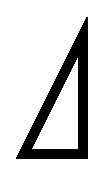
\includegraphics[height=11pt]{chapters/cap-partitura/torso-pe-esquerdo-tempo.eps},
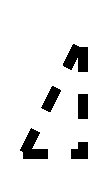
\includegraphics[height=11pt]{chapters/cap-partitura/torso-pe-esquerdo-indef.eps};
por outro lado os símbolos que representam que o pé que executa o movimento é o direito são:

\includegraphics[height=11pt]{chapters/cap-partitura/torso-pe-direito-contratempo.eps},
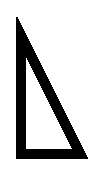
\includegraphics[height=11pt]{chapters/cap-partitura/torso-pe-direito-tempo.eps},
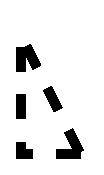
\includegraphics[height=11pt]{chapters/cap-partitura/torso-pe-direito-indef.eps};

\begin{abc}[name=chickchicktum1]
X: 1 % start of header
K: C % scale: C major
M:2/2
T: Chick-Chik Tum
V:1 clef=treble name="Instrumento 1" sname="Inst. 1"
V:2 clef=treble name="Instrumento 2" sname="Inst. 2"
[V:1] "Chik"G4 "Tum"E4 | "Chik"G4 "Tum"E4 |
[V:2] z2"Chik"G2 z4 | z2"Chik"G2 z4 |
\end{abc}

A Tabela \ref{tab:simbolospe}
\begin{table}[!hbt]
\caption{Tempos de espera apos levar o peso do corpo.}
\begin{center}
\begin{tabular}{|l |l | l |}
\hline
Tempo de espera  & Pé esquerdo & Pé direito \\
\hline
\hline
Médio tempo  & 

\includegraphics[height=11pt]{chapters/cap-partitura/torso-pe-esquerdo-contratempo.eps}   & 

\includegraphics[height=11pt]{chapters/cap-partitura/torso-pe-direito-contratempo.eps}   \\
\hline
Tempo  & 
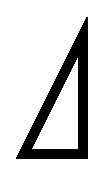
\includegraphics[height=11pt]{chapters/cap-partitura/torso-pe-esquerdo-tempo.eps}   & 
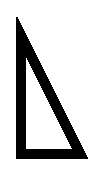
\includegraphics[height=11pt]{chapters/cap-partitura/torso-pe-direito-tempo.eps}   \\
\hline
Indefinido & 
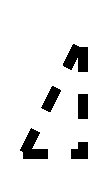
\includegraphics[height=11pt]{chapters/cap-partitura/torso-pe-esquerdo-indef.eps}   & 
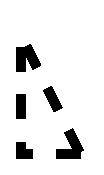
\includegraphics[height=11pt]{chapters/cap-partitura/torso-pe-direito-indef.eps}   \\
\hline
\hline
\end{tabular}
\end{center}
\label{tab:simbolospe}
\end{table}


%----------------------------------------------------------------------------------------
%	PART
%----------------------------------------------------------------------------------------

\part{Movimentos básicos}

%----------------------------------------------------------------------------------------
%	CHAPTERS
%----------------------------------------------------------------------------------------

%----------------------------------------------------------------------------------------
%	CHAPTER 2
%----------------------------------------------------------------------------------------

\chapter{Movimentos básicos na samba de gafieira}

\section{Frente trás}\index{Frente trás}

\section{Balanço}\index{Balanço}

\section{Cruzado}\index{Cruzado}




%----------------------------------------------------------------------------------------
%	PART
%----------------------------------------------------------------------------------------

\part{Outros exemplos}


%----------------------------------------------------------------------------------------
%	CHAPTER 
%----------------------------------------------------------------------------------------

%----------------------------------------------------------------------------------------
%	CHAPTER 3
%----------------------------------------------------------------------------------------

\chapterimage{chapter_head_1.pdf} % Chapter heading image

\chapter{Presenting Information}

\section{Table}\index{Table}

\begin{figure}[h]
\centering
\includegraphics[scale=0.5]{chapters/cap-exemplos/placeholder}
\caption{Figure caption}
\end{figure}



%----------------------------------------------------------------------------------------
%	BIBLIOGRAPHY
%----------------------------------------------------------------------------------------

\chapter*{Bibliografia}
\addcontentsline{toc}{chapter}{\textcolor{ocre}{Bibliography}}
\printbibliography[heading=bibempty]


%----------------------------------------------------------------------------------------
%	INDEX
%----------------------------------------------------------------------------------------

\cleardoublepage
\phantomsection
\setlength{\columnsep}{0.75cm}
\addcontentsline{toc}{chapter}{\textcolor{ocre}{Index}}
\printindex

%----------------------------------------------------------------------------------------

\end{document}
